%% March 2018
%%%%%%%%%%%%%%%%%%%%%%%%%%%%%%%%%%%%%%%%%%%%%%%%%%%%%%%%%%%%%%%%%%%%%%%%%%%%
% AGUJournalTemplate.tex: this template file is for articles formatted with LaTeX
%
% This file includes commands and instructions
% given in the order necessary to produce a final output that will
% satisfy AGU requirements, including customized APA reference formatting.
%
% You may copy this file and give it your
% article name, and enter your text.
%
%%%%%%%%%%%%%%%%%%%%%%%%%%%%%%%%%%%%%%%%%%%%%%%%%%%%%%%%%%%%%%%%%%%%%%%%%%%%
% PLEASE DO NOT USE YOUR OWN MACROS
% DO NOT USE \newcommand, \renewcommand, or \def, etc.
%
% FOR FIGURES, DO NOT USE \psfrag or \subfigure.
% DO NOT USE \psfrag or \subfigure commands.
%%%%%%%%%%%%%%%%%%%%%%%%%%%%%%%%%%%%%%%%%%%%%%%%%%%%%%%%%%%%%%%%%%%%%%%%%%%%
%
% Step 1: Set the \documentclass
%
% There are two options for article format:
%
% PLEASE USE THE DRAFT OPTION TO SUBMIT YOUR PAPERS.
% The draft option produces double spaced output.
%

%% To submit your paper:
\documentclass[draft,linenumbers]{agujournal2018}
\usepackage{apacite}
\usepackage{natbib}
\usepackage{amsmath}
\usepackage{multirow}
\usepackage{threeparttable}
\usepackage{url} %this package should fix any errors with URLs in refs.

\linespread{1.5}

%%%%%%%

% uncomment the line above to use the TrackChanges package to mark revisions if needed.
% The trackchanges package adds five new LaTeX commands:
%
%  \note[editor]{The note}
%  \annote[editor]{Text to annotate}{The note}
%  \add[editor]{Text to add}
%  \remove[editor]{Text to remove}
%  \change[editor]{Text to remove}{Text to add}
%
% complete documentation is here: http://trackchanges.sourceforge.net/
%%%%%%%

\draftfalse

% Now, type in the journal name: \journalname{<Journal Name>}

% ie, \journalname{Journal of Geophysical Research}
%% Choose from this list of Journals:
%
% JGR-Atmospheres
% JGR-Biogeosciences
% JGR-Earth Surface
% JGR-Oceans
% JGR-Planets
% JGR-Solid Earth
% JGR-Space Physics
% Global Biochemical Cycles
% Geophysical Research Letters
% Paleoceanography
% Radio Science
% Reviews of Geophysics
% Tectonics
% Space Weather
% Water Resource Research
% Geochemistry, Geophysics, Geosystems
% Journal of Advances in Modeling Earth Systems (JAMES)
% Earth's Future
% Earth and Space Science
% Geohealth
%

\journalname{Geophysical Journal International}

\begin{document}

%% ------------------------------------------------------------------------ %%
%  Title
%
% (A title should be specific, informative, and brief. Use
% abbreviations only if they are defined in the abstract. Titles that
% start with general keywords then specific terms are optimized in
% searches)
%
%% ------------------------------------------------------------------------ %%

% Example: \title{This is a test title}

\title{Stress concentration in the Central and Southeastern US seismic zones due to upper mantle heterogeneities} 
%% ------------------------------------------------------------------------ %%
%
%  AUTHORS AND AFFILIATIONS
%
%% ------------------------------------------------------------------------ %%

% Authors are individuals who have significantly contributed to the
% research and preparation of the article. Group authors are allowed, if
% each author in the group is separately identified in an appendix.)

% List authors by first name or initial followed by last name and
% separated by commas. Use \affil{} to number affiliations, and
% \thanks{} for author notes.
% Additional author notes should be indicated with \thanks{} (for
% example, for current addresses).

% Example: \authors{A. B. Author\affil{1}\thanks{Current address, Antartica}, B. C. Author\affil{2,3}, and D. E.
% Author\affil{3,4}\thanks{Also funded by Monsanto.}}

\authors{Arushi Saxena, Eunseo Choi, Christine A. Powell and Khurram S. Aslam}


% \affiliation{1}{First Affiliation}
% \affiliation{2}{Second Affiliation}
% \affiliation{3}{Third Affiliation}
% \affiliation{4}{Fourth Affiliation}

\affiliation{}{Center for Earthquake Research and Information, University of Memphis}
%(repeat as many times as is necessary)

%% Corresponding Author:
% Corresponding author mailing address and e-mail address:

% (include name and email addresses of the corresponding author.  More
% than one corresponding author is allowed in this LaTeX file and for
% publication; but only one corresponding author is allowed in our
% editorial system.)

% Example: \correspondingauthor{First and Last Name}{email@address.edu}

\correspondingauthor{Arushi Saxena}{asaxena@memphis.edu}

%% Keypoints, final entry on title page.

% Example:
% \begin{keypoints}
% \item	List up to three key points (at least one is required)
% \item	Key Points summarize the main points and conclusions of the article
% \item	Each must be 100 characters or less with no special characters or punctuation
% \end{keypoints}

%  List up to three key points (at least one is required)
%  Key Points summarize the main points and conclusions of the article
%  Each must be 100 characters or less with no special characters or punctuation

\begin{keypoints}
\item Numerical models reveal stress concentration from upper mantle velocity heterogeneity below seismic zones in the Central and Eastern US.
\item Lithospheric drip increases Coulomb stresses at the Eastern Tennessee and New Madrid seismic zones. 
\item Favorable preexisting faults along with deep upper mantle  heterogeneity could lead to earthquake generation in the Central and Eastern US.
\end{keypoints}

%% ------------------------------------------------------------------------ %%
%
%  ABSTRACT
%
% A good abstract will begin with a short description of the problem
% being addressed, briefly describe the new data or analyses, then
% briefly states the main conclusion(s) and how they are supported and
% uncertainties.
%% ------------------------------------------------------------------------ %%

%% \begin{abstract} starts the second page

\begin{abstract}
Sources of stress responsible for earthquakes occurring in the Central and Eastern US (CEUS) include not only far-field plate boundary forces but also various local contributions. In this study, we model stress distributions due to heterogeneities in the upper mantle beneath the CEUS including a high-velocity feature identified as a lithospheric drip in a recent regional P wave tomography study. We acquire velocity and stress distributions from numerical models for instantaneous three-dimensional mantle flow. Mantle flow in our models is driven by heterogeneous buoyancy arising from a temperature field converted from the P-wave velocities. The temperature field is utilized in the dislocation-diffusion creep rheology assumed in the models. When only the upper mantle heterogeneities are included in a model,  differential and Coulomb stress for the dominant fault geometries oriented for failure showed greater magnitudes at some of the seismic zones in the CEUS than in other regions. The model with the lithospheric drip and homogeneous mantle revealed that stress concentrates only in the vicinity of the drip which includes the Eastern Tennessee Seismic Zone and the northeast arm of the New Madrid Seismic Zone. Our modeling results suggest that the upper mantle heterogeneities below the CEUS have stress concentration effects and are likely to promote earthquake generation at preexisting faults in the region's seismic zones. However, assuming a range of theoretical fault orientations and dips, the most favorable fault geometry for failure from our models are not identical to the fault geometries inferred in the previous observational studies, suggesting additional factors for earthquake generation in this region. %Moreover, these heterogeneities increase the Coulomb stress at preexisting faults in the seismic zones, generating earthquakes.

\end{abstract}


%% ------------------------------------------------------------------------ %%
%
%  TEXT
%
%% ------------------------------------------------------------------------ %%


\section{Introduction}
     
    The tectonic setting of the Central and Eastern US (CEUS) includes complex fault systems formed by two continent-scale episodes of rifting and collision~\citep[e.g.,][]{keller1983role, hoffman1989precambrian, thomas2006tectonic}. Within these systems, favorably oriented faults with respect to the present-day regional or local stresses can get reactivated, generating earthquakes~\citep[e.g.,][]{zoback1992stress, hurd2012intraplate}. Indeed, the CEUS is characterized by several intraplate seismic zones including the New Madrid Seismic Zone (NMSZ), the Eastern Tennessee Seismic Zone (ETSZ), the South Carolina Seismic Zone (SCSZ), the Giles County Seismic Zone (GCSZ) and the Central Virginia Seismic Zone (CVSZ) (Fig.~\ref{figone}). 
    
\begin{figure}[h!]
    \centering
    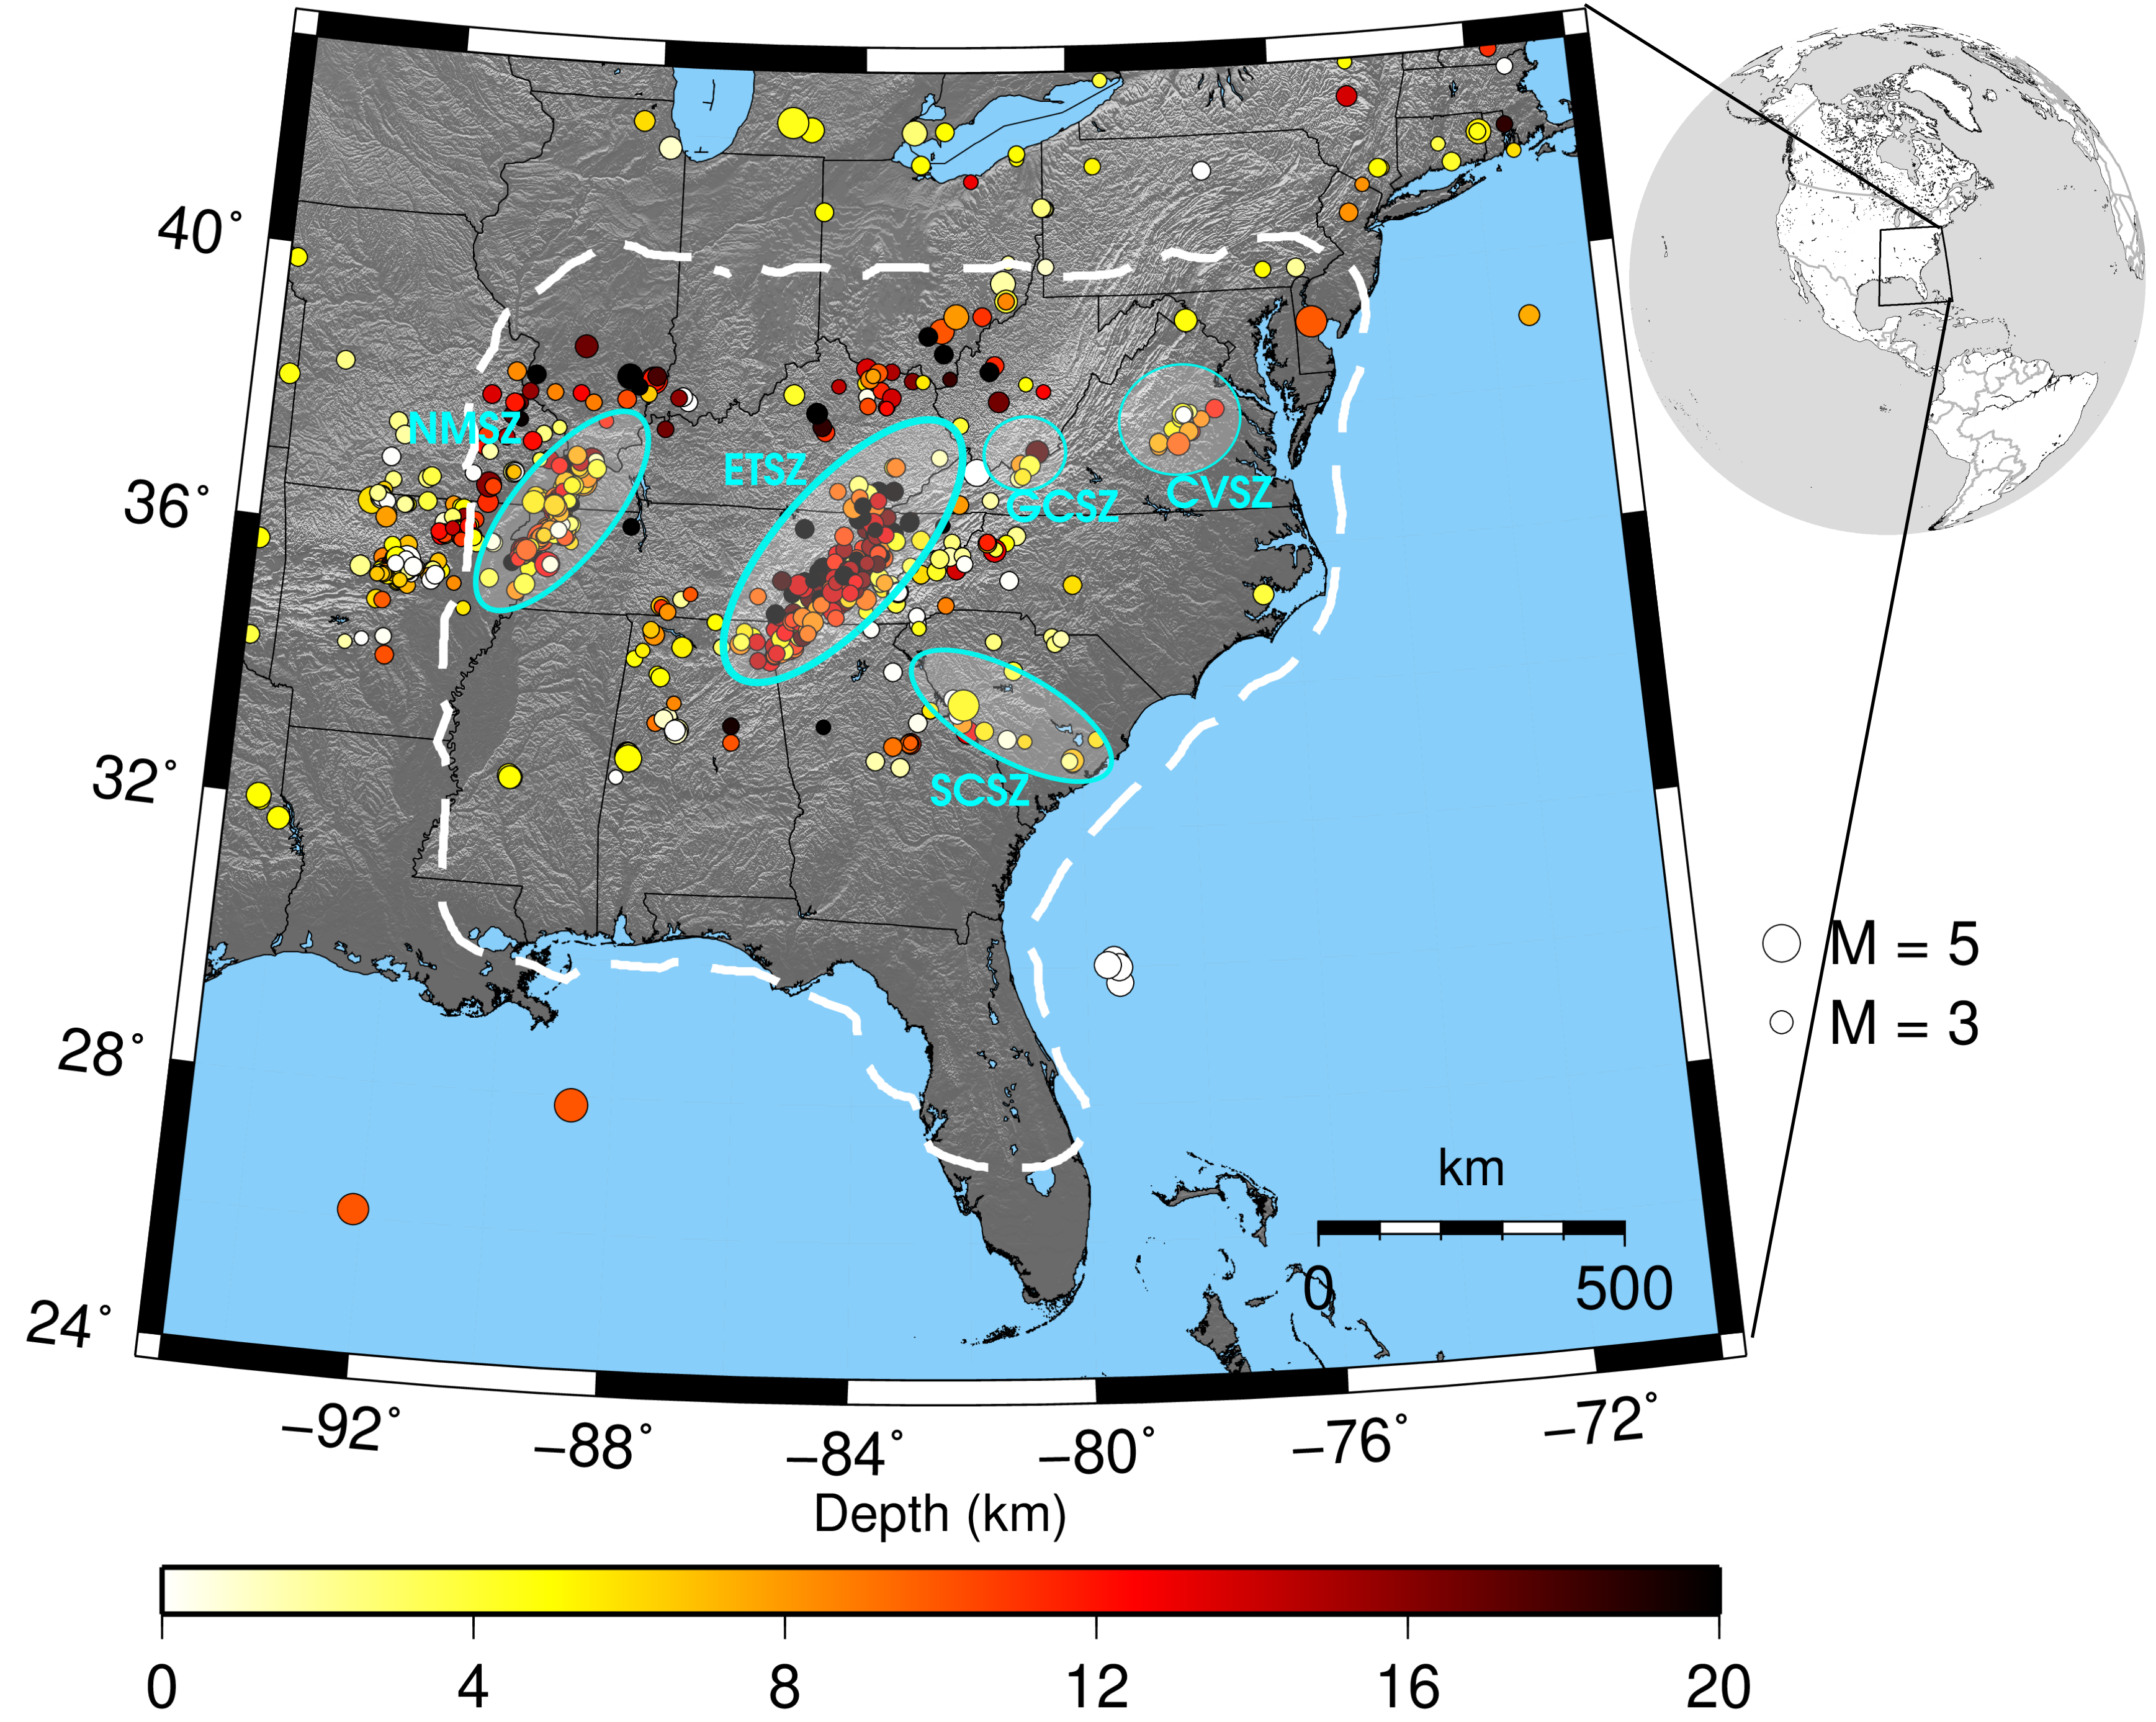
\includegraphics[width=32pc]{figures/seismicity_new.png}
    \caption{ A shaded relief map of the study area including the central and southeastern US seismic zones: New Madrid Seismic Zone (NMSZ), eastern Tennessee  Seismic Zone (ETSZ) South Carolina Seismic Zone (SCSZ), Giles County Seismic Zone (GCSZ) and Central Virginia Seismic Zone (CVSZ). White dashed line represents the well-sampled region in the tomography results by~\citet{Biryol_2016} at a depth 130 km. The earthquakes that occurred over the period December 2011 - December 2018 and had $M_{w} > 2.5$ are plotted as colored circles. The size and color of a circle represent the event's magnitude and depth. The earthquake catalog is obtained from the United States Geological Survey at \url{https://earthquake.usgs.gov/earthquakes/search/}.}
    \label{figone}
 \end{figure}
    
    Far from the tectonic plate boundaries and known to have low tectonic strain rates, earthquakes in the CEUS could be generated from local sub-lithospheric flow concentrating stress in the crust. Diverse origins of these local perturbations have been proposed, both crustal and upper mantle heterogeneity.~\citet{pollitz2001sinking} suggested a geodynamic model for the NMSZ consisting of a sinking mafic body in the weakened lower crust that can transfer stress into the overlying elastic crust. \citet{levandowski2016dense} showed that stress produced by a high density lower crust below the NMSZ interferes constructively with the far-field tectonic stress, causing optimal stress orientations for earthquake generation.~\citet{forte2007descent} showed that stress concentration below the NMSZ could be produced by the descent of the Farallon slab using a global geodynamic and seismic tomography based numerical model.~\citet{li2007stress} showed that lateral heterogeneity in the lithosphere could concentrate stress in the crust of the intraplate seismic zones of the CEUS.~\citet{chen2014crust} and~\citet{nyamwandha2016joint} independently observed a low P-wave velocity zone at 50-200 km depths below the NMSZ. This was interpreted as a weak zone that acts as a conduit for stress transfer into the crust.~\citet{becker2015western}  utilized the shear wave tomography model to compute temperature and density anomalies to set up numerical models, and found that the lithospheric heterogeneity plays a crucial role in predicting the intraplate seismicity for the Western US.  
    
Similar considerations of crustal and mantle stress sources are yet to be made for other CEUS seismic zones such as the ETSZ, SCSZ, GCSZ, and CVSZ. In a recent high-resolution P-wave tomography study, \citet{Biryol_2016} found positive velocity anomalies in the upper mantle beneath the area in-between the ETSZ and the NMSZ at depths of 200 to 660 km, and interpreted them as foundering lithosphere. They further speculated that, since the NMSZ and ETSZ coincide with the boundary of lithosphere thinned by the drip, they are weakened by the underlying hot asthenosphere and thus prone to seismicity. 

In this study, we investigate the effects of the upper mantle heterogeneities found in the P-wave tomography study by~\citet{Biryol_2016} on the seismicity in the CEUS. We compute stress and topographic fields  arising from the mantle flow generated from the heterogeneous density variations converted from the tomography using instantaneous three-dimensional (3D) numerical models. %explaining the location of seismic zones and assessing the sources of their initiation \citep{zoback1992stress, king1994static, stein1999role, bowman2001accelerating}. 
Following previous studies that have demonstrated correlation between differential stress~\citep[e.g.,][]{baird2010relationship, zhan2016stress},  deviatoric stresses~\citep[e.g.,][]{levandowski2016dense}, or topographic changes~\citep{becker2015western} with the observed intraplate seismicity, 
% These stress indicators are useful for  observing the stress distribution within the brittle crust. 
we will consider contributions of the upper mantle heterogeneity to these stress fields and discuss the slip tendency of faults in the seismic zones based on the Coulomb failure criterion~\citep[e.g.,][]{king1994static, freed2005earthquake, li2007stress}. \citet{ghosh2019role} took a similar approach to explaining the intraplate seismicity in the CEUS but our study differs in the scale of heterogeneity investigated. \citet{ghosh2019role} invoked long-wavelength lateral variations in viscosity structure  which are dependent on the age of lithosphere, and the location of plate boundaries. In contrast, we consider short-wavelength viscosity contrasts originating from the high-resolution heterogeneities in the upper mantle imaged in~\citet{Biryol_2016}\rq{}s tomography model. 


\section{Seismic tomography and upper mantle heterogeneities}

The tomography study by \citet{Biryol_2016} is based on direct P and PKPdf (P wave turning in the inner core) residual travel times for IASP91~\citep{kennett1991traveltimes}. The data are collected from 514 stations in the study region (Fig. \ref{figone}) for 753 teleseismic earthquakes occurring between 2011 to 2015 with moment magnitude, Mw $> 5.5$. The discretized model grid has a lateral extent of 30 km in the center and 45 km along the boundary of the domain. The depth extent of the grid is from 36 km to 915 km and consists of 21 layers, but we are only interested in the features extending down to 660 km for this study. The tomographic inversion algorithm is described in detail in the supplementary information by~\citet{Biryol_2016}. Only model nodes with high quality (hit points) are used, and therefore, only model results deeper than 60 km depth are interpreted by~\citet{Biryol_2016}.
    
    Biryol et al. (2016) evaluate their inversion results with resolution tests. The well-sampled region in the tomographic inversion shows high-velocity anomalies with a mean amplitude of 1.9\%, which are interpreted as lithospheric foundering (Fig.~\ref{fig_tomo}). The vertical cross-sections in Fig.~\ref{fig_tomo} show that these anomalies start at $\sim$ 200 km depth with lateral dimensions of  $\sim$ $2^\circ$ and extend to 660 km where they widen to $\sim$ $3^\circ$ (marked in Fig.~\ref{fig_tomo}A). According to the synthetic anomaly tests, the supposed foundering lithospheric drip with these amplitudes and dimensions should be reliably resolved.
%
\begin{figure}[h!]
    \centering
    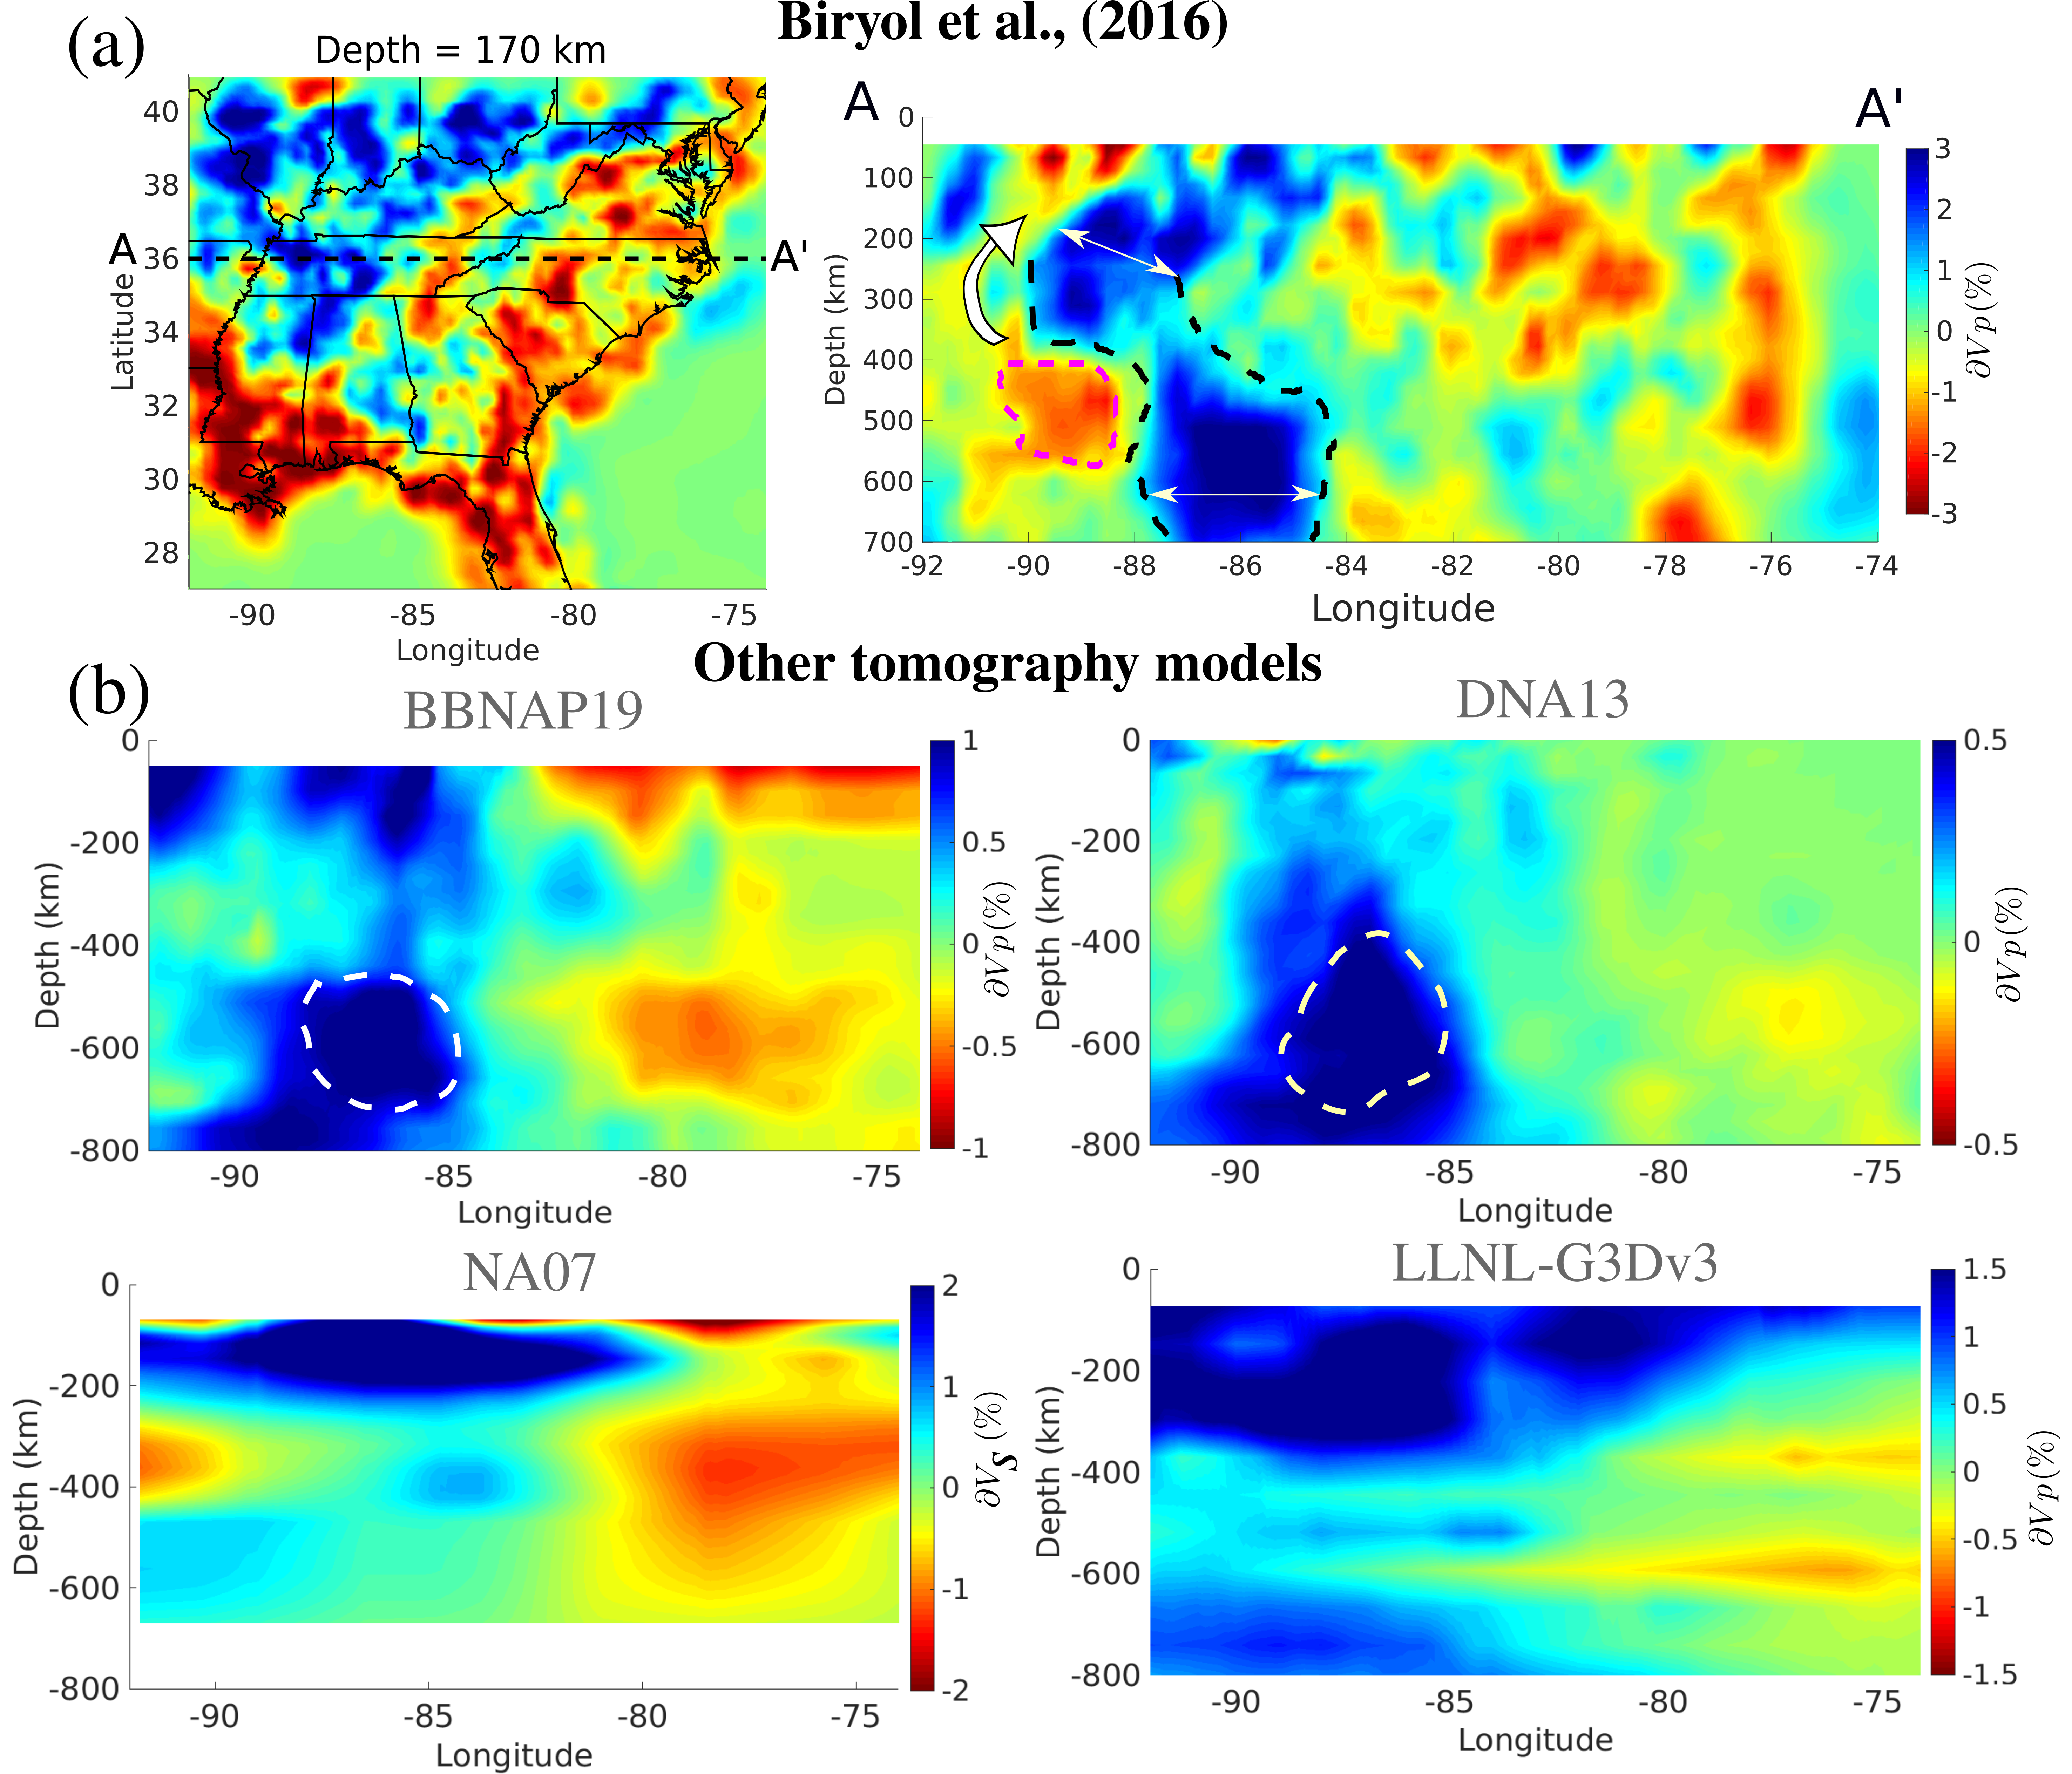
\includegraphics[width=1\linewidth]{figures/updated_tomography.png}
    \caption{Tomography results from~\citet{Biryol_2016} used in this study, and other published tomography models for comparison. (a) P wave tomography results by~\citet{Biryol_2016} for a layer at 170 km and a cross-section through latitude 36$\circ$ for comparison with other tomography models. Dashed black line on the cross-sections marks the approximate boundaries of the high-density anomalies interpreted as a foundering lithospheric root. Dashed magenta line indicates the low-velocity region interpreted by~\citet{Biryol_2016} as asthenospheric return flow due to the foundering lithosphere and the white arrow shows the direction of the return flow as speculated by~\citet{Biryol_2016}. (b) Other published tomography models along the 36$^\circ$ latitude cross-section. The white dashed lines in the BBNAP19 model and the DNA13 model show the outline of the high-density anomaly observed in detail by \citet{Biryol_2016}.}
    \label{fig_tomo}
 \end{figure}
 
We also assess the performance of the regional tomography model by~\citet{Biryol_2016} using global and  contiguous US tomography models. Fig.~\ref{fig_tomo} shows the vertical cross-section along latitude 36$^\circ$ for four different tomography models: BNAP19~\citep[P-wave tomography model of the continental US concentrating on the upper mantle structure by][]{boyce2019variable}, DNA13~\citep[P-wave and S-wave velocity model for the contiguous US by][]{porritt2014seismic}, NA07~\citep[S-wave velocity model of the upper mantle in the North America by][]{bedle2009s}, and LLNL-G3Dv3~\citep[Global P-wave tomography model by][]{simmons2012llnl}. The high-velocity anomalies observed by~\citet{Biryol_2016} can also be seen in the BBNAP19 and the DNA13 tomography models (dashed white lines in Fig.~\ref{fig_tomo}). However, the color scales in both the BBNAP19 ($\partial Vp=\pm1$\%) and DNA13 ($\partial Vp=\pm0.5$\%) models clearly show that the high-velocity anomaly is resolved in much higher detail($\partial Vp=\pm3$\%) in the~\citet{Biryol_2016} model. A correspondence between the ~\citet{Biryol_2016} model and models, NA07 and LLNL-G3Dv3, is not observed. This is understandable as NA07 is a shear wave velocity model while~\citet{Biryol_2016} utilize P-wave traveltimes, and  LLNL-G3Dv3 is a global tomography model extending to the core-mantle boundary, which makes it difficult to resolve regional anomalies. 


\section{Modeling instantaneous mantle flow}
%    Inputs for our mantle flow models include temperature and density fields converted from the velocity anomalies. The velocity-to-temperature conversion method we adopt~\citet{Cammarano2003} takes into account the effects of anelasticity, compositional variations, and phase changes. An effective power-law rheology is assumed to be \annote[EC]{a combination} of diffusion and dislocation creep. 
%To facilitate interpretation of the effects of high-density anomalies found in the upper mantle, we choose a reference model in which temperature \annote[EC]{below the model}{What does this mean?} is laterally homogeneous \note[EC]{What about radially?}. Models based on the tomography are compared with the reference model in terms of differential stress and Coulomb stress changes. The latter is computed for selected values of near-surface fault strike and dip. We also examine dynamic topography caused by the mantle flow induced by the sinking denser material.
    
\subsection{Temperature Calculations} \label{temp_var}
    Inferring temperature from the seismic velocity anomalies has primary importance for our modeling approach because it will determine both the driving buoyancy force and the viscous resistance. We follow \citet{Cammarano2003}'s approach to calculate temperatures from the seismic velocity anomalies. This approach takes into account the effects of anharmonicity (i.e. elasticity), anelasticity and the phase transition at 410 km depth. Inversion of seismic tomography results to a temperature field is commonly regarded as a non-linear problem due to the shear anelasticity of seismic waves \citep{minster1981model, karato1993importance, sobolev1996upper, Goes_2000, artemieva2004shear} and non-linear sensitivity of elastic moduli and their pressure derivatives to temperature \citep{duffy1989seismic, anderson1992high, Cammarano2003, stixrude2005thermodynamics}. The presence of melt or water may also introduce non-linearity in temperature effects on seismic velocities~\citep{Karato_1998} but the effects of melt and fluids are not considered in this study because of the lack of high heat flow and other substantial evidence for melting in this region of the mantle~\citep{blackwell2006assessment}. Our inversion procedure is fully detailed in Appendix A.
%
%Both anharmonic and anelastic effects on seismic velocities \remove[EC]{, which are discontinuous at the 410 km phase transition,} are taken into account in our inversion for temperature.\note[EC]{The previous sentence is redundant with the intro paragraph of this section. Probably you don't need it.} 
    
The average scaling of velocity anomalies to the inverted temperatures with depth is shown in Fig.~\ref{fig_temp}. The non-linear sensitivity of Vp anomalies to temperature perturbations with depth can be seen from Fig.~\ref{fig_temp}. The average P-wave velocity (Vp) sensitivity to temperature is found to be $-$0.80 \% per 100$^\circ$K and $-$0.62 \% per 100$^\circ$K at two representative depth layers 200 km and 605 km, respectively. These values are consistent with those in~\citep{Cammarano2003}: $-$0.75$\pm$0.15 \% per 100$^\circ$K and $-$0.65 \% per 100$^\circ$K at the same depths, along the mantle adiabats 1300$^{\circ}$C and 1600$^{\circ}$C, respectively, used in this study. The velocity anomalies, along with the inverted temperatures for depths of 200 km and 605 km are shown in Fig.~S1.
%
\begin{figure}[ht]
    \centering
    \includegraphics[width=0.6\linewidth]{figures/depth_average.png}
    \caption{The calculated depth-averaged P-wave velocity sensitivity to temperature. See text for details of calculations.} 
    \label{fig_temp}
 \end{figure}

\subsection{Model Setup}
  %  \note[EC]{Although a nice summary, this paragraph seems redundant and doesn't fit in the Model Setup section.} We calculate the stress field associated with an instantaneous viscous mantle flow. The mantle flow is driven by thermal buoyancy arising from the heterogeneous temperature distribution converted from the P-wave tomography by \citet{Biryol_2016} as described above. Model inputs, density, and viscosity distributions are computed based on the converted temperatures. 
    
    We compute velocity and stress fields that are in equilibrium with heterogeneous buoyancy forces arising from the heterogeneous distribution of temperature-dependent density. For this calculation, we use an open-source finite element code, ASPECT version 2.0.0~\citep{heister_aspect_methods2,KHB12,aspect-doi-v2.0.0}. ASPECT can solve the equations for the conservation of mass, momentum, and energy using an adaptive finite element method for a variety of rock rheologies. 
    
     Our model domain is laterally bounded by longitudes, 71$^{\circ}$W and 95.5$^{\circ}$W and by latitudes, 23$^{\circ}$N and 43$^{\circ}$N. The depth range is from 0 to 660 km (Fig.~\ref{fig_model}). Since the tomography model considers only the mantle starting from a depth of 36 km, we assume a temperature distribution appropriate for the crust. We divide the crust into four depth layers such that the temperature is constant in each layer (Fig.~\ref{fig_model}). Our choice of discretization represents the crustal structure appropriately and is not important here since we are interested in the deeper ($>$ 40 km) heterogeneity. The domain is discretized into 0.512 million hexahedral elements with a 0.15$^{\circ}$ resolution in longitude, 0.125$^{\circ}$ in latitude, and 35 km in depth. This spatial resolution is similar to that of the tomography and thus sufficient for resolving the mantle velocity structure shown by the tomography model. 

We assessed mesh resolution effects by running a model with a twice finer mesh having 2.048 million elements and found that differences in the results were small, amounting to a relative error of 2\% in the velocity field. All the model results presented in this study are thus based on the coarse mesh for computational efficiency. We also tested a model with an additional lateral area of 5$^{\circ}$ by 5$^{\circ}$ surrounding our domain to asses boundary effects. The overall resultant velocity and stress field are similar to those for the smaller model domain, but the magnitude of the calculated stress and velocity field at our depth of interest (15 km) near the boundaries is smaller by 10-15 \% because the viscous effect of the same heterogeneity is now spread over a larger area. However, since the seismic zones are sufficiently far from the model domain boundaries, we show only the results for the smaller domain.
%
\begin{figure}[ht]
    \centering
    \includegraphics[width=0.75\linewidth]{figures/model_figure.png}
    \caption{Model setup with the computed rheology based on the regional tomography by \citet{Biryol_2016} and the boundary conditions applied. Gray isosurface represents P-wave anomalies $>$ 2 \% in the region interpreted as lithospheric foundering. Instantaneous flow along slice AA' passing through the ETSZ and NMSZ is discussed in Fig. \ref{velocity_pattern}. Black lines indicate the state boundaries and red dots are epicenters for the earthquake catalog used in Fig. \ref{figone}. Temperature depth profile of the crust is shown on the left.}
    \label{fig_model}
\end{figure}

Upper mantle flow is assumed to occur by a dislocation creep at low temperatures relative to the melting temperatures of mantle rocks and by a diffusion creep at higher temperatures~\citep[e.g.,][]{gordon1967thermally} with respect to the melting temperatures. Our model employs both dislocation and diffusion creep with each type having different contributions depending on the temperature and pressure. In this rheology model, the effective viscosity ($\eta_{\text{eff}}$) is computed as~\citep{billen2007rheologic}:
%
\begin{align}
    \eta_{\text{i}} &= \frac{1}{2} A^{-\frac{1}{n_i}} d^\frac{m_i}{n_i} \dot{\varepsilon_i}^{\frac{1-n_i}{n_i}} \exp\left(\frac{E_i + PV_i}{n_iRT}\right),\ i=\text{diff or dis}, \\
    \eta_{\text{eff}} &= \left(\frac{1}{\eta^\text{diff}} + \frac{1}{\eta^\text{dis}}\right)^{-1},
\end{align}
%
where diff and dis denote diffusion and dislocation creep, $A_i$ is the pre-exponential factor, $n_i$ is the power law exponent, $d$ is the grain size, $m_i$ is the grain size exponent, $\dot{\varepsilon}$ is the second invariant of the strain rate tensor, $R$ is the gas constant, $T$ is temperature obtained from the inversion of the Vp anomalies, $P$ is pressure, and $E_i$ and $V_i$ are the activation energy and volume, respectively. All the parameter values used in this study are given in Table~\ref{table_model}.
%
\begin{table}[ht] 
    \caption{Values for dislocation and diffusion creep}
    \centering
    \begin{tabular}{l c c c c}
    \hline
     Parameter  & Symbol & Unit & Diffusion Creep & Dislocation Creep  \\
    \hline
      Pre-exponential factor$^a$ & $A$ & $s^{-1}$ & 1.5 $\times$ 10$^{-16}$ & 0.3 $\times$ 10$^{-22}$   \\
      Power law exponent$^a$ & $n$ & & 1 & 3.5  \\
      Grain size exponent$^a$  & $m$ & & 2 & 0   \\
      Activation energy$^a$  & $E$ & kJ/mol & 300 & 530   \\
      Activation volume$^a$  & $V$ & cm$^3$/mol & 6 & 20 \\
      Grain size$^b$         & $d$ & mm & 5 & 5 \\
    \hline
    \multicolumn{5}{l}{$^{a}$\citet{karato1993rheology}. $^b$Approximate value for olivine~\citep{karato1984grain}.}
    \end{tabular}
    \label{table_model}
\end{table}

The bottom boundary at 660 km has the free-slip condition~\citep[e.g.,][]{arcay2007slab, billen2007rheologic, quinquis2011role}. For side boundaries, we tested our model with both free-slip and no-slip conditions and verified that the velocity fields at the seismic zones have the same pattern with up to 5\% magnitude difference. In this study, we only show the results for the no-slip conditions. We let the top boundary be a free surface that can develop topography in response to the instantaneous flow in the mantle. 
%I don't think you need explain this: based on \citet{kaus2010stabilization} free surface stabilization implemented in ASPECT) 

\subsection{Earthquake predictors}
We compute various measures for earthquakes for our model setup (Fig.~\ref{fig_model}): gravitational potential energy, dynamic topography, and rate of change of dynamic topography. We also compute different stress indicators, differential stress, observed Coulomb stress, and optimal Coulomb stress to isolate the effects of upper mantle heterogeneity (discussed in the following subsections). 

The computed earthquake measures are quantified for their predictive power to estimate the seismicity of our region using Molchan curves and their associated skill, S, following the work by~\citet{becker2015western}. Each curve is plotted for the range of values of a predictor, and for each value $p$, fraction number of earthquakes that lie within the region where predictor values are less than that value, $p$, are plotted against the fraction of predictor values below $p$. The skill for each predictor is computed as the area of the curve above the Molchan curve minus 0.5, such that a pure random predictor has $S=0$, a pure correlation has $S=0.5$, and a pure anti-correlation has $S=-0.5$.  

\subsubsection{Gravitational potential energy}
We calculate gravitational potential energy per unit area in our model following the thin-sheet approximation described in~\citet{ghosh2009contribution} as:
\begin{equation}
GPE = \int_{-h}^{L} z \rho(z) g dz,
\end{equation}
where $\rho(z)$ is the density at a depth z, g is the acceleration due to gravity taken as 9.8 g/cc, h is the surface topography, and L is the assumed compensation depth used as 200 km. We choose this depth to represent the approximate thickness of the lithosphere for the continents~\citep{mckenzie2005thermal}. We use CRUST1.0~\citep{laske2013update} model for crustal thickness and density distribution, and a homogeneous lithosphere with a representative density value of 3250 kg/m$^3$~\citep{becker2014static}. 

\subsubsection{Dynamic topography and its rate}
The dynamic topography for our model is computed in ASPECT, and it represents the radial stress at the surface due to the mantle flow generated from the buoyancy effects of densities based on the heterogeneous temperature distribution. We compute the rate of dynamic topography by computing the change in dynamic topography between our instantaneous model and our model run forward in time for 10,000 years~\citep{becker2015western}.  

\subsubsection{Differential and Coulomb stress changes}
We define static changes in Coulomb stress ($\Delta C$) of a model with respect to another model as the difference in Coulomb Failure Function (CFF)~\citep{king1994static}:
%
\begin{equation} \label{eq4}
    \Delta C = \Delta \tau - \mu' \Delta \sigma_n,
\end{equation}
%
where $\Delta \tau$ and $\Delta\sigma_n$ are the difference between the models in shear (positive in the direction of slip) and normal (positive when compressive) stress, respectively, for a particular fault orientation, and $\mu'$ is the effective coefficient of friction after accounting for pore pressure. Since we do not have sufficient constraints on the effective friction coefficients for the faults in the study area, we use a value of 0.6 based on the study by~\citet{hurd2012intraplate}. The details of the Coulomb stress computation are in Appendix B. Differential stress, $\sigma_{\text{diff}} \equiv \sigma_{1}-\sigma_{3}$, is compared between different models with a similarly defined quantity, $\Delta \sigma_{\text{diff}}$.


To facilitate comparison of models with and without the local upper-mantle heterogeneity, delineated by the velocity anomaly isosurface in Fig.~\ref{fig_model}, we denote our reference model (Fig.~\ref{fig_model}) with tomography-based temperatures plus the reference geotherm as HT (HeTerogeneous), a model with the reference geotherm in the upper mantle as HM (HoMogeneous), and a model identical with HT except that the temperature within the foundering lithosphere is replaced with the reference geotherm values as HR (Heterogeneous but having no Root). HT$-$HM represents the contributions from the upper mantle heterogeneity, while HT$-$HR shows only the contribution of the high-velocity structure interpreted as the foundering drip. Fig.~\ref{model_differences} shows a cross-section of the tomography illustrative of these model setups.  Coulomb stress changes, $\Delta$C$_{HT-HM}$ and $\Delta$C$_{HT-HR}$, indicate whether and how much the stress field in the model HT would promote the slip tendency of a fault relative to stress fields in HM and HR. For instance, a positive $\Delta$C$_{HT-HM}$ for a fault geometry and a sense of motion means that the mantle heterogeneities considered in HT promote the failure of the fault relative to the laterally homogeneous mantle (HM). 

\begin{figure}[h!]
    \centering
    \includegraphics[width=\linewidth]{figures/model_differences_updated.png}
    \caption{Cross-section along latitude=$36^\circ$ across model setups for which stress calculations are done in this study. HT, HM, and HR represent the HeTerogeneous, Homogeneous Mantle and Homogeneous Root models, respectively. The models, HT$-$HM and HT$-$HR isolates the effects of upper mantle heterogeneity and lithospheric drip, respectively.}
    \label{model_differences}
\end{figure}

We calculate $\Delta C$ and $\Delta \sigma_{\text{diff}}$ for HT$-$HM and HT$-$HR, and analyze the results at the seismic zones ETSZ, SCSZ, CVSZ, GCSZ, and the NMSZ (shown in Fig.~\ref{zones}) which are contained in the well-resolved region in the~\citet{Biryol_2016} tomography. CFF values are computed for the selected fault geometries based on the focal mechanisms and earthquake relocations at 15 km depth in all the seismic zones (Table \ref{table_fault}).
%
\begin{table}
\caption{Seismic Zones$^{*}$ and their associated dominant fault geometries}
\centering
\begin{tabular}{ l l l l } 
    \hline
    Seismic Zone & Strike, Dip & Sense of motion & Reference \\
    \hline
    NMSZ\_NE &  N$10^\circ$E, 90$^\circ$ & right-lateral & \citet{chiu1992imaging, shumway2008focal} \\ 
    NMSZ\_RF & N$167^\circ$E, 30$^\circ$SW & thrust & \citet{csontos2008new} \\ 
    \multirow{2}{2em} {ETSZ\ \ \ } & \multirow{2}{7em}{1- N$10^\circ$E, 90$^\circ$; 2- E-W, 90$^\circ$} &  \multirow{2}{6em}{right-lateral; left-lateral} &  \multirow{2}{20em} {\citet{chapman1997statistical, cooley2015new, powell2016grenville}} \\ & & & \\
    %ETSZ & N$10^\circ$E, 90$^\circ$ & right-lateral & \citet{chapman1997statistical, cooley2015new, powell2016grenville} \\
    %         & E-W, 90$^\circ$              & left-lateral    &   \\
    GCSZ & E-W, 90$^\circ$ & left-lateral  & \citet{munsey1985focal} \\ 
    CVSZ & N$30^\circ$E, 50$^\circ$SE & thrust  & \citet{wu2015aftershock}  \\ 
    SCSZ & N$180^\circ$E, 40$^\circ$W & thrust & \citet{chapman2016modern}\\    
    \hline
\end{tabular}
 \begin{tablenotes}
    \begin {small}
        \item[1] $^{*}$ NMSZ\_NE: North eastern arm of New Madrid Seismic Zone; NMSZ\_RF: Reelfoot fault of the New Madrid Seismic Zone; ETSZ: Eastern Tennessee Seismic Zone; GCSZ: Giles County Seismic Zone; CVSZ: Central Virginia Seismic Zone; SCSZ: South Carolina Seismic Zone. 
     \end{small}
  \end{tablenotes}
\label{table_fault}
\end{table}

\subsubsection{Optimal Coulomb stress}
We define the optimal fault orientation as the one maximizing the Coulomb stress changes of HT relative to HM ($\Delta C_{\text{HT}-\text{HM}}$), and for HT relative to HR ($\Delta C_{\text{HT}-\text{HR}}$). We calculate the optimal fault orientation using a grid search over strikes from N$90^\circ$E to S$90^\circ$E and dips from 10$^\circ$ to 90$^\circ$ at an interval of $10^\circ$ for the possible senses of motion, right- and left-lateral strike-slip, normal and thrust faulting. The optimal fault orientation could also be calculated analytically using two successive stress rotations (one to align a plane at a strike angle and then a rotation to a fault dip), and then solving for the strike and sip angles that maximize the $\Delta C$. Since we are also interested in the $\Delta C$ distribution over the range of strikes and dips, we use the grid search method.

%%%
\section{Model results}
Several indicators are computed for our models to correlate with seismicity, which are quantified using Molchan analysis~\citep{becker2015western}, and the visual distribution of all the indicators is presented in the supplementary material. The Molchan curves for the earthquake predictors are computed for all the model points in the subregion marked in Fig.~\ref{zones}, which includes all the seismic zones of the CEUS investigated in this study. However, since each seismic zone has a unique fault geometry, only the points within each seismic zone are accounted for calculating the Mochan curves of the Coulomb stress and the optimal Coulomb stress indicators. 
%
\begin{figure}
\centering
	\includegraphics[width=0.6\linewidth]{figures/seismic_zones.png}
	\caption{Model points (red) at each seismic zone for which the Molchan curves of Coulomb stress and the optimal Coulomb stress are computed. The box BB'CC' indicates the region for which all the other Molchan curves are calculated. }
	\label{zones}
\end{figure}

We compute three earthquake indicators at the surface for our reference model, which is based on the tomography converted temperatures and viscosities (Fig.~\ref{fig_model}), gravitational potential energy, dynamic topography, and rate of dynamic topography (Fig. S1). These indicators are quantified using Molchan curves and their associated skill is calculated in Fig.~\ref{ref_skill}.
%
\begin{figure}
\centering
	\includegraphics[width=0.65\linewidth]{figures/reference_model_results.png}
	\caption{Molchan curves for the indicators, $h_{dyn}$: dynamic topography, $dh_{dyn}/dt$: rate of dynamic topography change, and $GPE$: gravitational potential energy, computed for the HeTerogeneous (HT) model. The computed skill for each indicator is mentioned in the legend with gray. The diagonal black line represents a purely random indicator. }
	\label{ref_skill}
\end{figure}

Fig.~\ref{ref_skill} shows that both the dynamic topography and its rate show negative skill for prediction of earthquakes, such that the rate of dynamic topography has a much lower skill, $S=-0.16$ comparted to the skill of dynamic topography, $S=-0.06$. The gravitational potential energy (GPE) shows a high positive skill of $S=0.24$. This indicates that many earthquakes could be found in areas where the GPE has high values. Contrarily, a large number of earthquakes overlie regions with low values of rate of dynamic topography, while not much correlation can be seen between the earthquake distribution and the dynamic topography.

To account for stress effects from only upper-mantle lateral heterogeneity ($>$ 60 km depth), we compute the stress indicators for the HT$-$HM model at a depth of 15 km, at which seismicity in the study area is most frequent~\citep[e.g.,][]{mazzotti2010state}. We consider three indicators of stress: differential stress, Coulomb stress at the observed fault geometries (Table~\ref{table_fault}), and optimal Coulomb stress (Fig. S2), and plot their corresponding Molchan curves and skills in Fig.~\ref{ht_hm_skill}. All the stress indicators for HT$-$HM show a positive correlation with the observed seismicity, implying that a large number of earthquakes are found in the regions where these stresses are high. 
%
\begin{figure}
\centering
	\includegraphics[width=0.5\linewidth]{figures/ht_hm_updated.png}
	\caption{Molchan curves for the indicators, $\Delta \sigma_{diff}$: change in differential stress, $\Delta C$: change in Coulomb stress for the observed fault orientations at each seismic zone, and $\Delta C_{opt}$ Coulomb stress change for the optimal fault geometry where the shear stress is maximum, computed for the HT$-$HM  model. The computed skill for each indicator is mentioned in the legend with gray. The diagonal black line represents a purely random indicator. }
	\label{ht_hm_skill}
\end{figure}

Stress indicators computed for HT$-$HR model, which isolates only the effects from the lithospheric drip, are similarly plotted in Fig.~\ref{ht_hr_skill}. It can be inferred from Fig.~\ref{ht_hr_skill} that the differential stress negatively correlates with the observed earthquake distribution. The Coulomb stress at the observed fault geometries (Table~\ref{table_fault}) show minimal correlation with the seismicity. On the other hand, the optimal Coulomb stress show high positive correlation with the observed seismicity.
%
\begin{figure}
\centering
	\includegraphics[width=0.6\linewidth]{figures/ht_hr_updated.png}
	\caption{Same as Fig.~\ref{ht_hm_skill} but for HT$-$HR.}
	\label{ht_hr_skill}
\end{figure}

%
    %%%%%
\section{Discussion}

%    In this study, we investigate the stress effects due to upper mantle heterogeneity, $>$ 200 km depth, and isolated lithospheric instability on the intraplate seismicity of the CEUS using numerical models based on the temperatures calculated from the \citet{Biryol_2016} tomography results. Many possible stress concentrators in the CEUS have been proposed to explain the seismicity \citep[e.g.,][]{levandowski2016dense, zhan2016stress} but analysis done here invoking deeper upper mantle structures and impact collectively on the seismicity in the CEUS has not been done before. 
Our results from the Molchan analysis on the tomography-based numerical model suggests that Gravitational Potential Energy (GPE) is the best predictor to explain the seismicity distribution (Fig.~\ref{ref_skill}).  Contrarily to the similar study by~\citet{becker2015western} for the Western US, in which change their computed rate of dynamic topography shows a high correlation with the intraplate seismicity, we find that the dynamic topography and its rate show a negative correlation with the seismicity of the CEUS  (Fig.~\ref{ref_skill}). The GPE values represent the vertical stress field arising from the laterally-varying lithospheric structure and crustal densities and its structure, implying that the structural heterogeneity is an important factor to consider for understanding the earthquake generation in the CEUS. However, the dynamic topography indicative of the mantle flow generated from the buoyancy effects of the tomography-based density anomalies does not appear to have a correlation with the seismicity pattern in the CEUS.
    
Changes in differential stress ($\Delta \sigma_{\text{diff}}$) and the Coulomb stress ($\Delta$C) for the cases HT$-$HM and HT$-$HR quantify how the upper-mantle heterogeneity and the lithospheric drip, respectively, can contribute to the seismicity in the ETSZ, GCSZ, CVSZ, SCSZ, and NMSZ (see Fig. \ref{zones} for their locations).
$\Delta\sigma_{diff}^{\text{HT}-\text{HM}}$ involves the combined effects of all the mantle heterogeneities relative to the laterally homogeneous reference mantle and shows a positive correlation with the observed seismicity  (Fig.~\ref{ht_hm_skill} ). On the other hand, the lithospheric drip alone has a negative correlation with the earthquake locations in this region (Fig.~\ref{ht_hr_skill} ). Although the positive values of differential stress changes suggest an increased potential for seismicity, even the greatest value of $\Delta\sigma_{diff}^{\text{HT}-\text{HM}}$, $\sim$ 30 MPa in the ETSZ (Fig. S2), is an order of magnitude less for that required for the nucleation of earthquakes at crustal depths of 10-20 km~\citep[e.g.][]{sibson1990rupture}. This deficiency in magnitude requires other contributions for explaining the seismicity in the CEUS like weak existing faults created during the past several Wilson cycles~\citep{thomas2006tectonic}. From our Coulomb stress change calculations for the observed fault geometries of the seismic zones (Table~\ref{table_fault}), we find that these faults are more loaded towards failure  in the heterogeneous upper mantle revealed by the tomography (Fig.~\ref{ht_hm_skill})  than in the laterally uniform one (Fig.~\ref{ht_hr_skill}). As expected from the definition of the optimal Coulomb stress ($\Delta C_{opt}$), the skill for both the cases HT$-$HM and HT$-$HR at each seismic is maximum amongst all the stress indicators (Fig.~\ref{ht_hm_skill}, ~\ref{ht_hr_skill}). 
       
    
    %The Coulomb stress change is calculated at the selected fault orientations determined from previous studies on focal mechanism and earthquake hypocentral relocation in these seismic zones \citep[e.g.,][]{cooley2015new, powell2016grenville, munsey1985focal, chiu1992imaging}. In HT$-$HM, ETSZ, GCSZ and northeastern arm of NMSZ show an increase in Coulomb stress for the proposed fault orientation in these regions and CVSZ shows a weak positive increase while SCSZ overlies in the stress shadow, i.e. negative Coulomb stress change. Conversely, HT$-$HR does not show strong correlation between seismiciy and the Coulomb stress increase at all seismic zones except NMSZ.
    
     The optimally oriented fault planes computed for model isolating all the upper-mantle heterogeneity, HT$-$HM,  do not perfectly coincide with the focal mechanism solutions in the seismic zones (Fig.~\ref{summary}). There are several reasons for the mismatch between the focal mechanism solutions and the optimal fault orientations for our models in the seismic zones (Fig.~\ref{summary}) . Firstly, the focal mechanisms investigated in this study for each of the seismic zones are not unique; there are other proposed focal mechanisms documented in the literature, but we only select focal planes for each seismic zone that are most prevalent. Moreover, at some seismic zones such as the SCSZ and the CVSZ, the seismicity is spatially diffused so that a single mechanism cannot describe the entire zone~\citep{johnson2014earthquake, munsey1985focal, madabhushi1993fault}.  Secondly, the presence of upper mantle heterogeneity is not the only contributing factor for stress concentration in the CEUS. Other factors such as a dense sinking body in a weak lower crust as proposed by \citet{Pollitz_2001} or weak lower crust or upper mantle embedded in an elastic lithosphere by \citet{Kenner_2000a} or isostatic response from deglaciation of Laurentia by ~\citet{Grollimund_2001}, may also play a role in affecting stresses at 10-20 km depths. Thirdly, most of the earthquakes in the CEUS occur at depths $<$ 20 km~\citep[e.g.,][]{bollinger1985seismicity, chiu1992imaging, powell2016grenville} on reactivated faults formed from past Wilson cycles~\citep{thomas2006tectonic, wolin2012mineral}. However, the mantle tomography model used in our study does not provide constraints on the geometry and strength of the shallow seismogenic faults created in the past. Lastly, our model does not account for any tectonic stresses since our focus is on the local stress perturbations from the upper mantle. In reality, the effects of plate motion, as included by~\citet{zhan2016stress} and \citet{levandowski2016dense}, will influence the near-surface stress field.
%
\begin{figure}[ht]
    \centering
    \includegraphics[width=0.8\linewidth]{figures/summ_stress.png}
    \caption{Proposed fault planes from other studies based on focal mechanism and earthquake hypocenters versus fault planes at which $\Delta$C$_{HT-HM}$ is maximum. The markers represent each of the seimic zones: New Madrid Seismic Zone (NMSZ), Eastern Tennessse Seismic Zone (ETSZ) South Carolina Seismic Zone (SCSZ), Giles County Seismic Zone (GCSZ) and Central Virginia Seismic Zone (CVSZ). The sense of fault slip is indicated with the color of the marker as thrust(T), right-lateral strike-slip (SS, RL), left-lateral strike slip (SS, LL) and normal (N). Encircled markers represent the orientations maximizing $\Delta$C$_{HT-HM}$. A double-ended arrow pairs the observed and modeled fault orientations for each seismic zone.}
    \label{summary}
\end{figure}
 
     %The important result of our study is the increase in the Coulomb stress in the active CEUS seismic zones due to the presence of the upper mantle heterogeneity.
%    which is computed using $R'=(\sigma_2-\sigma_3)/(\sigma_1-\sigma_3)$ (here, $\sigma_1>\sigma_2>\sigma_3$ are the principal stress components and $\sigma_1$ is most compressive), and the faulting style
%
%\add[AS]{The direction of maximum horizontal stress} (S$_H$) is an useful indicator to interpret seismicity~\citep[e.g.,][]{assumpccao1985fault}, crustal anisotropy~\citep[e.g.,][]{boness2004stress} and plate motion~\citep[e.g.,][]{richardson1992ridge} \note[EC]{For some reason, these references are not properly processed on my side. Please see if they look fine on your PDF and if not, correct the corresponding bibtex entries (or citatiations)}. We compute S$_H$ and faulting style for our tomography-based heterogeneous model, HT, in Fig.~\ref{sigma1} and compare them with the proposed S$_H$ and faulting style from a recent stress inversion study by~\citet{levandowski2018updated}. 
%
The directions of maximum horizontal stress (S$_H$) computed from the model HT roughly match those obtained by~\citet{levandowski2018updated} in all the seismic zones but the ETSZ (Fig.~\ref{sigma1}).  S$_{H}$ based on HT is NNW-SSE in the ETSZ differing from the NE-SW direction determined using focal mechanism solutions by~\citet{levandowski2018updated} and by~\citet{mazzotti2010state}. This is not surprising as faulting in the ETSZ may be strongly influenced by density anomalies in the lower crust inherited from past tectonic events~\citep{levandowski2018updated}, which are not accounted in this study.

The distribution of stress regime parameter, $R$,~\citep{delvaux1997paleostress,simpson1997quantifying}, computed based on the model HT, shows that the dominant faulting styles are thrust for the NMSZ\_NE, and oblique-thrust for the GCSZ (Fig.~\ref{sigma1}). These stress regimes are consistent with the proposed faulting styles in~\citet{levandowski2018updated} for these zones, but differ from the selected studies in Table~\ref{table_fault} which suggest strike-slip for the GCSZ and the NMSZ\_NE.  
% R varies from 0 for radial extension, through normal, strike-slip, and reverse faulting to radial contractionlevandowski2018updated at R=3~\citep{delvaux1997paleostress, simpson1997quantifying}. 
The HT model predicts normal faulting at the SCSZ and the CVSZ. These zones are associated with thrust faulting in~\citet{levandowski2018updated}, and the studies mentioned in Table~\ref{table_fault}. This discrepancy between the modeled and predicted faulting style at the CVSZ and the SCSZ occurs because our model does not account for compressive tectonic stresses due to ridge push, which are highest at these zones. Within the ETSZ, a strike-slip mechanism has been suggested by other studies~\citep[Table 2][]{mazzotti2010state, powell2016grenville} which agrees with our model result, but differs with \citet{levandowski2018updated} who find normal faulting in the ETSZ.  This discrepancy may be because~\citet{levandowski2018updated} consider new focal mechanism data in their stress inversions indicating a propensity for normal faulting in the ETSZ~\citep[also found in][]{cooley2015new}.

\begin{figure}[h!]
    \centering
    \includegraphics[width=0.75\linewidth]{figures/sigma1.png}
    \caption{Maximum horizontal stress directions (S$_H$) at all the seismic zones for the heterogeneous (HT) model (black lines) overlain over the stress regime (R) computed using the principal stresses at these seismic zones.  }
    \label{sigma1}
\end{figure}

%    The stresses in our model arise from instantaneous flow due to the upper mantle heterogeneity. Fig. \ref{velocity_pattern} shows the velocity field at slice AA$^{\prime}$ (marked in Fig \ref{fig_model}) in the model HT due to heterogeneous density computed from temperatures based on the tomography study by \citet{Biryol_2016}. 
A broad downward flow is found below both the NMSZ and ETSZ in the velocity field (Fig. \ref{velocity_pattern}) on the cross-section AA$^{\prime}$ of the model HT (marked in Fig \ref{fig_model}). The descending flow induces upwellings along the edges of the model domain. The upwellings are observed at the surface as features F$_1$ and F$_2$ marked in Fig. S2. The broadly downward flow due to the lithospheric drip is not consistent with the asthenospheric upwelling that~\citet{Biryol_2016} proposed would occur as a counter-flow to the drip. However, the asthenopsheric upwelling cannot be reliably rejected because the velocity field in our model depends on various parameters including the viscosity of the asthenosphere and the boundary conditions. Lower viscosity of the asthenosphere, for instance, would reduce the lateral extent of the downward drag by the lithospheric drip such that the region beneath the NMSZ might not be affected as strongly as in the current model. We ran models with only diffusion creep and only dislocation creep and found similar flow directions  bu a different flow law might alter the flow pattern around the high-density foundering lithosphere. A model with depth dependent viscosity with a high viscosity layer in the transition zone would inhibit a downward flow from the high-density lithospheric drip, making the velocity vectors turn at shallower depths.

~\citet{forte2007descent} presented viscous numerical models based on the joint inversion of seismic and geodynamic data and observed a downward vertical flow beneath the NMSZ, which could generate intraplate seismicity. Comparing our flow field with the results from~\citet{forte2007descent}, we can see a similar vertical flow at depths 300-500 km, but the velocity pattern above these depths differ significantly. A possible reason for the mismatch is that our study incorporates a regional tomography model (\citep{Biryol_2016}), while Forte et al., (2007) model is based on a global model focusing on much larger wavelength anomalies.
%However, even with lower viscosity asthenosphere, it is still unlikely that the buoyancy effects produced by the localized low-velocity anomaly below the NMSZ (Fig. \ref{fig_tomo}) would counteract the downward pull from the much more significant positive anomaly lithospheric drip.
%    
\begin{figure}[ht]
    \centering
    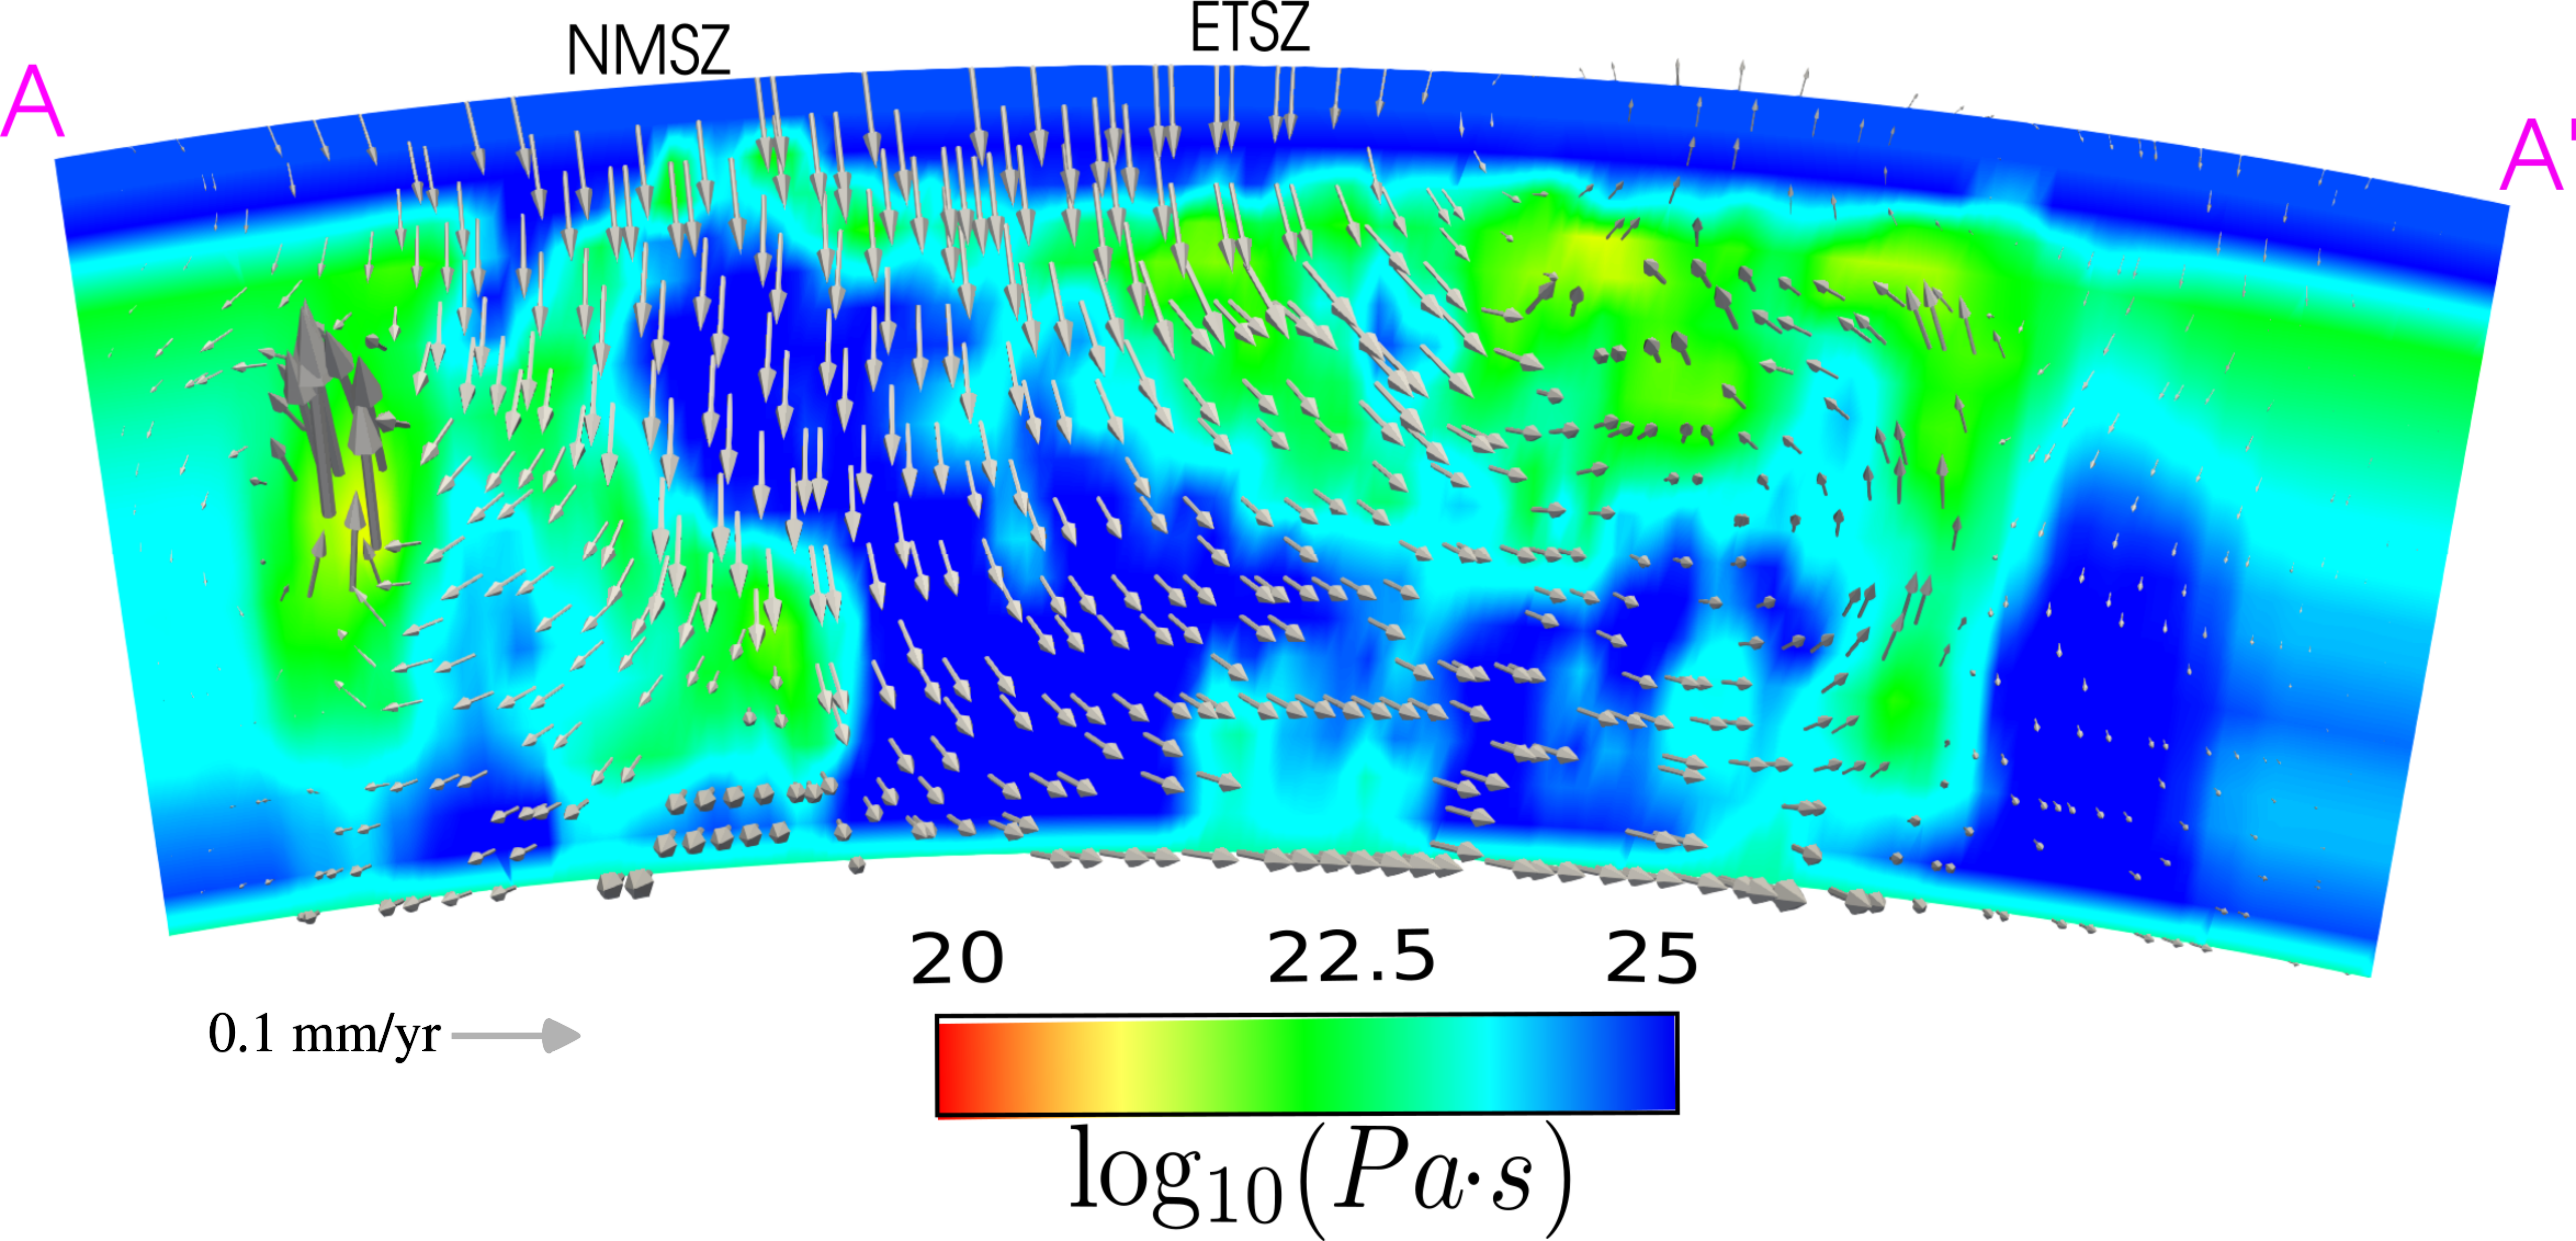
\includegraphics[width=0.9\linewidth]{figures/velocity_pattern.png}
    \caption{Velocity (arrows) and viscosity fields from the model HT on the slice AA$^{\prime}$ (marked in Fig \ref{fig_model}). The extreme high-velocity vectors observed west of the NMSZ and out of the plane are from the upward return flow due to the downward pull of the lithospheric drip and are likely an artifact due to fixed boundary conditions at the sides.}
%and the viscosity distribution computed from the temperatures based on the tomography by \citet{Biryol_2016}. 
%}
    \label{velocity_pattern}
\end{figure}     
%
This study focuses on the contribution from local stress perturbations on the seismicity of the CEUS, but another likely mechanism to explain the earthquakes in this region is the presence of spatially limited weak zones activated under tectonic stresses. This idea has been studied previously by~\citet{Kenner_2000a,  zhan2016stress} for the NMSZ.~\citet{Kenner_2000a} proposed a model with a weak lower crustal zone within an elastic lithosphere that acts as a local source of stress concentration from the far-field stresses. Similarly, based on a regional tomography model by~\citet{pollitz2014seismic},~\citet{zhan2016stress} found that weak upper mantle inferred from low seismic velocities can focus stress in the NMSZ crust. In order to test this, we apply the regional stress direction,  northeast-southwest compressive stress for the CEUS~\citep{zoback1989tectonic}, in our tomography-based heterogeneous model (Fig.~\ref{model_differences}). However, our differential stress calculations with the plate boundary stress directions do not show correlation with the observed seismic zones. There is a big shortcoming in this result that is the absence of the spatially limited crustal weak zones (fault zones) in our model. This complexity is outside the scope of this study and is not addressed here further.     
     
Time dependent modeling will be needed to address the mechanism for the origin of a foundering drip in the CEUS. It has been proposed by \cite{Biryol_2016} that the lithospheric foundering could have started due to Rayleigh-Taylor instability beginning from the presence of an ecologized root as proposed by \citet{le2006mantle} in the western US. Such an investigation in this region would call for more sophisticated techniques such as backward advection modeling~\citep[e.g.,][]{conrad2003seismic}, quasi-reversibility~\citep{glivsovic2016new}, or adjoint methods~\citep[e.g.,][]{bunge2003mantle, liu2008reconstructing} for the calculation of initial conditions on temperature, viscosity and density, which has not been done in this study.

 It is also possible that the dense high-velocity mantle feature is part of the subducted Farallon slab below this region~\citep{schmid2002fate, mooney2010north, sigloch2008two, schmandt2010complex, sigloch2011mantle}. ~\citet{schmid2002fate} used kinematic thermal modeling to track the subduction history of the Farallon slab and found that the Farallon lithosphere continues to the central US and is still a negative thermal anomaly observable in the seismic tomography studies.~\citet{mooney2010north} computed the gravity signal from the upper mantle for North America and observed a large gravity high in the southeastern US, which they attributed to the east-dipping Farallon slab.~\citet{schmandt2010complex} present Vp and Vs tomographic images for the western US and interpret their positive velocity anomalies in the Rockies as the eastward dipping segmented Farallon slab.~\citet{sigloch2008two, sigloch2011mantle} present P-wave tomography for North America until about 1800 km depth, and interpret the high-velocity anomaly in the CEUS at the mantle transition depths as a stagnant fragment of the Farallon slab.  We do not comment on the origin of this high-velocity feature but follow the naming convention by \citet{Biryol_2016} as a drip in this study. Additional observations such as low dynamic topography at the surface would be required to confirm if the high velocity is indeed attached to the lithosphere or is a remnant Farallon slab.
  
\section{Conclusions}

The role of local stress perturbations has been studied previously to explain the intraplate seismicity of the CEUS. In this study, we advance the understanding by utilizing the highest upper mantle resolution tomography study~\citep{Biryol_2016} till date and setup numerical models with laterally heterogeneous viscosity and density. We also explore the isolated effects of upper-mantle heterogeneity and a positive P-wave velocity anomaly, interpreted by \citet{Biryol_2016} as a lithospheric drip in our numerical models, which has not been examined before. We follow the novel Molchan analysis approach to quantify various earthquake metrics with their corresponding skills, $S$, following the work by~\citet{becker2015western} on the Western US. We compute earthquake predictors for our numerical model, such as rate of dynamic topography and gravitational potential energy, not been investigated in the previous studies.

Our analysis of various earthquake predictors to understand the seismicity in the CEUS has revealed that the lateral upper-mantle heterogeneity below this region plays a significant role in increasing the differential stress ($S=0.22$) and Coulomb stress ($S=0.27$) at observed fault geometries. Moreover, we also find that upper mantle structural heterogeneity and density anomalies measured using GPE ($S=0.24$) is important for understanding deformation in this region. The stress indicators for the model with lithospheric drip only do not show correspondence with the observed seismicity pattern. Therefore, our results provide a possible mechanism for reactivation of the faults in the intraplate seismicity of the CEUS. This, in turn, helps to better associate seismic hazard with the seismic zones in the CEUS.

\appendix
\section{Appendix: Seismic tomography inversion}


\begin{table}
\caption{Mineral physics data used in this study \tnote{1}}
\centering
\begin{tabular}{ l c c c c c c c c c } 
\hline
 \multirow{2}{3em}{Mineral} & \multirow{2}{3em}{$\rho$ (kg/m$^3$)} & \multirow{2}{3em}{$K_S$ (GPa)} & \multirow{2}{3em}{$\mu$  (GPa)}  & $K'$ & $\mu'$ &  \multirow{2}{4em}{$\partial K/\partial T$ (GPa/K)}  & \multirow{2}{4em}{$\partial \mu/\partial T$ (GPa/K)} & \multirow{2}{4em}{$a_0 (10^{-4})$} & \multirow{2}{4em}{$a_1 (10^{-7})$} \\ & & & & & & & & & \\
 \hline
  olivine  & 3222 & 129 &  81 & 4.2 & 1.4 & -0.017 & -0.014 & 0.20 &  0.139  \\
  orthopyroxene  & 3215 &  109 &  75 & 7 & 1.6 & -0.027 & -0.012 & 0.387 & 0.044 \\
  garnet  &  3565 & 171 & 92 & 4.4 & 1.4 & -0.019 & -0.01 & 0.099 & 0.116 \\
  wadsleyite  & 3472 & 172 & 121 & 4.5 & 1.5 & -0.014 & -0.014 & 0.232 &  0.0904 \\
  majorite  &  3565  & 171 & 92 & 4.4 & 1.4 & -0.019 & -0.01 &  0.0991 & 0.1165   \\
\hline
\end{tabular}
  \begin{tablenotes}
  \begin {small}
     \item[1] $\rho$: density, $K_S$: adiabatic bulk modulus, $\mu$: shear modulus, $K'$: pressure derivative of bulk modulus, $\mu'$: pressure derivative of shear modulus, $\partial K/\partial T$: bulk modulus derivative with temperature, $\partial \mu/\partial T$: shear modulus derivative with temperature, $a_0$, $a_1$ are constants in thermal expansivity, $\alpha = a_0 + a_1 T$. Values of elastic moduli and their derivatives are from \citet{Cammarano2003} and thermal expansivity are from \citet{saxena_data}.
     \end{small}
  \end{tablenotes}
 \label{table1}
\end{table}

The effects of composition at high temperature and pressure are incorporated in seismic velocity following \citet{Cammarano2003} in which the elastic moduli ($K$, $G$) and densities ($\rho$) at reference temperature $T_0$ and pressure $P_0$ are first extrapolated at high temperatures ($T$) and then adiabatically at high pressures ($P$) following finite-strain extrapolation \citep{duffy1989seismic}. The calculations are divided at pressures $~$12.5 GPa to account for phase transformation of olivine to $\beta$ spinel at 410 km. 

To calculate density at high pressures, a mantle adiabat with potential temperature ($T_{pot}$) $1300^o C$ was chosen for depths $\leq$ 410 km and $1600^o C $ for deeper depths up to 660 km. Strain ($\epsilon$) is first calculated at known pressures (based on PREM model by \citet{dziewonski1981preliminary}) using $K_0$, $G_0$ and their pressure derivatives, $K_S'$, $G'$  (Table \ref{table1}).  Reference density calculated at the potential temperature and zero pressure ($\rho(T_{pot}, P_0)$) is then used to get the density $\rho (P,T)$.

\begin{align*} 
    P &=  - (1 - 2\epsilon)^{5/2} \left[ 3K_0\, \epsilon + \frac{1}{2} \left( 9K_0 ( 4 - K_S' ) \right) \epsilon^2 \right], \\
    \epsilon &= \frac{1}{2} \left[ 1 - \left( \frac{\rho(T,P)}{\rho(T_{pot}, P_0)} \right) ^{2/3} \right] \\
    \rho(T_{pot}, P_0) &=  \rho(T_0, P_0) \, \exp \left( - \int_{T_0}^{T_{pot}} \alpha (T) dT \right)
\end{align*}
where thermal expansivity, $\alpha(T) = \alpha_0 + \alpha_1 T$ is truncated after the second term. Density changes due to temperature, $T$ from the reference geotherm, $T_o$ and pressure are calculated from above as:

\begin{equation}\label{den_der}
    \delta \rho = \rho(T_0, P_0) \text{exp} \left( - \int_{T_0}^{T} \alpha (T') dT' \right) \alpha(T) ) (T - T_o)
\end{equation}

Temperature dependence on $K$ $G$, is assumed linear while changes in $K_S'$, $G'$ is calculated from the procedure in \citep{duffy1989seismic} as: 

\begin{align*} 
    \delta M\vert_{T, P0} &= \frac{\partial M}{\partial T }  ( T - T_o )\\
    \delta M'\vert_{T, P_0} &=  \left( M'(T_0) \text{exp} \left[ \int_{T_0}^{T} \alpha (T) dT \right] \alpha(T) \right) ( T - T_o )  ,
\end{align*}
where $M$ is either $K$ or $G$, $\delta M$, $\delta M'$ are changes in elastic modulus and its  pressure derviate due to temperature $T$.

Elastic moduli changes are then evaluated at high pressures using second-order extrapolation order expansion \citep{duffy1989seismic}:

\begin{align} \label{M_der}
    \delta K + \frac{4}{3} \delta G &= ( 1 - 2 \epsilon)^{5/2} \left[ M_1 + \epsilon \left( 5 L_1 - 3 \frac{\partial K}{\partial T }  ( T - T_o ) \left[ K' + \frac{4}{3} G' \right] - 3K_0 M_2 \right)  \right], \\ 
    \text{where}, \hspace{0.5cm}
    M_1 &= \delta K\vert_{T, P0} + \frac{4}{3}\delta G\vert_{T, P0} ; \hspace{0.5cm}
    M_2 = \delta K'\vert_{T, P_0} + \frac{4}{3}\delta G'\vert_{T, P_0} \nonumber
\end{align}

The anharmonic velocity variations due to temperature and pressure are then calculated using \ref{den_der}, \ref{M_der} for each mineral and then averaged using Voigt (constant strain) averaging scheme for the reference composition, discontinuous across 410 km,  described in section \ref{temp_var}.

\begin{equation} \label{anh}
    \delta V \vert_{anh} = \frac{1}{2\sqrt{K_0 + 4/3 G_0} \sqrt{\rho_0}} \left[\delta K + \frac{4}{3} \delta G \right] - \frac{K_0 + 4/3 G_0}{1\rho_0^{3/2}} ( \delta \rho)
\end{equation} 

Frequency dependence (anelasticity) of velocity with temperature is incorporated following \citet{Goes_2000}:

\begin{align} \label{anel}
    \delta V \vert_{anel} &= Q_p^{-1} \frac{aH}{2 R T^2 \tan(\pi a/2)},\\
    Q_p^{-1} &= A \omega^{a} \exp \left[ \frac{a(H+PV)}{RT} \right] \frac{3Vp_{0}^{2}}{4Vs_{0}^{2}} \nonumber
\end{align}
Here, $\omega = 2\pi $, values of laboratory constants, $a = 0.15, A = 0.148$, activation energy $H = 500$ kJ/mol, volume $V = 20$ cm$^3$/mol are taken from \citet{sobolev1996upper}. $Vs_0$ and $Vp_0$ are S and P wave velocities from IASP91 \citep{kennett1991traveltimes}.

%We use the equation (\ref{anh}) to calculate anharmonic effects on seismic velocity.
The reference geotherm ($T_0$) for lithospheric (i.e., $<$ 200 km) depths is the one used in~\citep{Goes_2002} for eastern US and for greater depths, we follow Fig. 4.56 from~\citet{turcotte2014geodynamics} due to lack of evidence for regional geotherms at deeper depths. Thermal expansivity ($\alpha$) from~\citet{saxena_data} (see Table~\ref{table1}). We assume a reference composition of harzburgite, i.e., 83 \% olivine (ol), 15 \% orthopyroxene (opx), 2 \% garnet (gt)~\citep{mcdonough1998mineralogy} for depths 40 km to 410 km or pressure (P) $<$ 12.5 GPa. For depths from 410 km to 660 km, we use a reference composition of 60 \% Mg-wadsleyite and 40 \% Majorite~\citep{haggerty1995upper}. We use Burnman, a mineral physics toolbox~\citep{cottaar2014burnman}, to calculate the mantle adiabat with a potential temperature of 1300$^{\circ}$C for P $<$ 12.5 GPa, which is appropriate for continental lithosphere \citep{rudnick1998thermal} and 1600$^{\circ}$ for P $>$ 12.5 GPa~\citep{katsura2010adiabatic}. Values for bulk modulus ($K_S$), shear modulus (G) and density ($\rho$) for each mineral in the composite are taken from~\citet{Cammarano2003} and are listed in Table~\ref{table1}.

%Anelasticity is implemented using~\ref{anel} using the values given by~\citet{sobolev1996upper} 
We account for the anelastic effects on the seismic velocity by correcting for the power law dependence of frequency on seismic attenuation, $Q_p$. We use linear pressure dependence on activation enthalpy ($H(P)= H_0 + VP$, V is the activation volume) in calculating $Q_p$, (model 2 described in\citet{sobolev1996upper}). Another way to correct for pressure dependence on enthalpy is using melting temperature dependence, (model 1 in \citet{sobolev1996upper}, i.e., $H(P)= gRT_m$ where g is constant and $T_m$ is melting temperature). We use model 2 because we do not include the effects of melting in the seismic anomalies for the reasons discussed earlier. We use a value of 1 Hz for the frequency in the attenuation calculation.

The inversion procedure starts with an initial guess for temperature and updates the temperature values at all the observational points in the tomography until the difference of the calculated anomalies with the observed seismic anomalies is minimized. We also calculate temperatures accounting for uncertainties in the elastic moduli and their temperature derivatives as in~\citep{Cammarano2003}) and compare them with the results obtained here using the mean values given in Table \ref{table1}. Taking the maximum values of the elastic parameters reduces the temperature sensitivity such that the negative (positive) velocity anomaly decreases (increases) temperature by a small ($\pm$ 90 K) magnitude. On the other hand, minimum parameter values increase the temperature sensitivity, and therefore the range of temperatures obtained, by $\sim$ 180 K.

Our approach has several differences from that of~\citet{Cammarano2003}. Firstly, we invert velocity anomalies, not absolute velocities, for temperature anomalies, which are added to an assumed reference geotherm $T_o$. Secondly, we use the Voigt averaging scheme to calculate elastic moduli and density of the composite rock instead of the Hashin Shtrikman scheme used by~\citet{Cammarano2003}. Although the Voigt scheme is known to overestimate the converted values~\citep{watt_1976}, seismic velocities based on compositions averaged by the Voigt scheme, which is representative of the upper bound value for the composite~\citep{watt_1976}, and the Reuss scheme, which is representative of the  lower bound value for the composite~\citep{watt_1976}, shows less than 0.2 \% difference in magnitudes. Since this error is within the range of the tomography error \citep{Biryol_2016}, we use the computationally simpler Voigt scheme. Finally, elastic moduli at high pressures are extrapolated using second-order accuracy instead of third-order for simplicity in implementation of the inversion.

\section{Appendix: Coulomb stress calculation}

Stress tensors in the model outputs are given as Cartesian stress components with respect to $x$ and $y$ axes at 0$^{\circ}$ and 90$^{\circ}$ longitudes and on the equator. Stress tensors are transformed according to a rotation of the model domain by which the $z$ axis goes through the center of the domain. After this rotation, $x$ and $y$ axes approximately coincide with East and North as understood in the model. Stress tensors are further transformed such that $x$, $y$ and $z$ axes in the rotated Cartesian system coincide with a fault\rq{}s strike, up-dip and normal directions (Fig.~\ref{signs}). We follow the convention that strike is defined as the direction that puts a dipping fault plane on the right and dip angle changes between 0$^{\circ}$ and 90$^{\circ}$. %surface  is located at the  follow the right-hand rule such that dips are measured on the right side of the footwall facing the fault strike and 
In the final coordinate system, negative values of $\tau_{zx}$ and $\tau_{zy}$ correspond to right-lateral and down-dip sense of motion, respectively.
% High $\mu$ between 0.5 and 0.8 is associated with \annote[EC]{limited}{What do you mean?} fault cohesion and therefore, \annote[EC]{slip while lower values, i.e. 0-0.5 are generally taken for smooth sealed faults capable of larger slip accumulation}{The meaning of this sentence is not clear to me.} \citep{parsons1999stress}. 
%
\begin{figure}[h!]
    \centering
    \includegraphics[width=0.5\linewidth]{figures/sign_convention.png}
    \caption{Cartoon sketch showing the sign convention for the strike, dip, and normal to the fault surface. }
    \label{signs}
\end{figure}

%%%

\acknowledgments
We thank Dr. Berk Biryol for sharing his tomography results used for modeling in this study. We also thank the Computational Infrastructure for Geodynamics (geodynamics.org) which is funded by the National Science Foundation under award EAR-0949446 and EAR-1550901 for supporting the development of ASPECT.

%%%%%

%% ------------------------------------------------------------------------ %%
%% References and Citations

%%%%%%%%%%%%%%%%%%%%%%%%%%%%%%%%%%%%%%%%%%%%%%%
% BibTeX is preferred:
%
\bibliography{agusample}
%
% no need to specify bibliographystyle
%%%%%%%%%%%%%%%%%%%%%%%%%%%%%%%%%%%%%%%%%%%%%%%



% Please use ONLY \citet and \citep for reference citations.
% DO NOT use other cite commands (e.g., \cite, \citeyear, \nocite, \citealp, etc.).
%% Example \citet and \citep:
%  ...as shown by \citet{Boug10}, \citet{Buiz07}, \citet{Fra10},
%  \citet{Ghel00}, and \citet{Leit74}.

%  ...as shown by \citep{Boug10}, \citep{Buiz07}, \citep{Fra10},
%  \citep{Ghel00, Leit74}.

%  ...has been shown \citep [e.g.,][]{Boug10,Buiz07,Fra10}.


\end{document}

 Although the stress distribution overlies the seismicity well, our numerical models for the stress computations are only constrained by the temperature conversions from the seismic tomography results by \citet{Biryol_2016} and any errors in the calculated temperature will be transmitted to viscosity and to our stress calculations. 
%
%% ------------------------------------------------------------------------ %%
%
%  IN-TEXT LISTS
%
%% ------------------------------------------------------------------------ %%
%
% Do not use bulleted lists; enumerated lists are okay.
% \begin{enumerate}
% \item
% \item
% \item
% \end{enumerate}
%


%%%%%%%%%topography

%    We examined the topography generated due to the mantle flow generated from the upper mantle heterogeneity in Fig. \ref{topo_res}. 
We calculated residual topography in our study region following the approach by \citet{becker2014static} for the isostatic and dynamic topography for the western US. We first calculate the isostatic topography. We use CRUST1.0~\citep{laske2013update} for crustal thickness and density (Fig. \ref{topo_res}a) and LITHO1.0~\citep{pasyanos2014litho1} for lithospheric thickness variations (Fig. \ref{topo_res}b). We assume a constant lithospheric density of 3300 kg/m$^3$ and a constant asthenosphere density of 3250 kg/m$^3$. These values are reasonable for a density contrast between the lithosphere and asthenosphere~\citep[e.g.,][]{bonnardot2008numerical, ito2011probing}. Although the crustal contribution to the topography is about 10 times more dominant than the lithosphere for these density values, the residual topography highs are preferentially associated with the very thinned lithospheric locations (Fig. \ref{topo_res}c), which have greater influence than the crustal thickness variations. We also plot the residual topography due to the density distribution based on the~\citet{Biryol_2016} tomography in Fig.~\ref{topo_res}d. 
%   
\begin{figure}[h!]
    \centering
    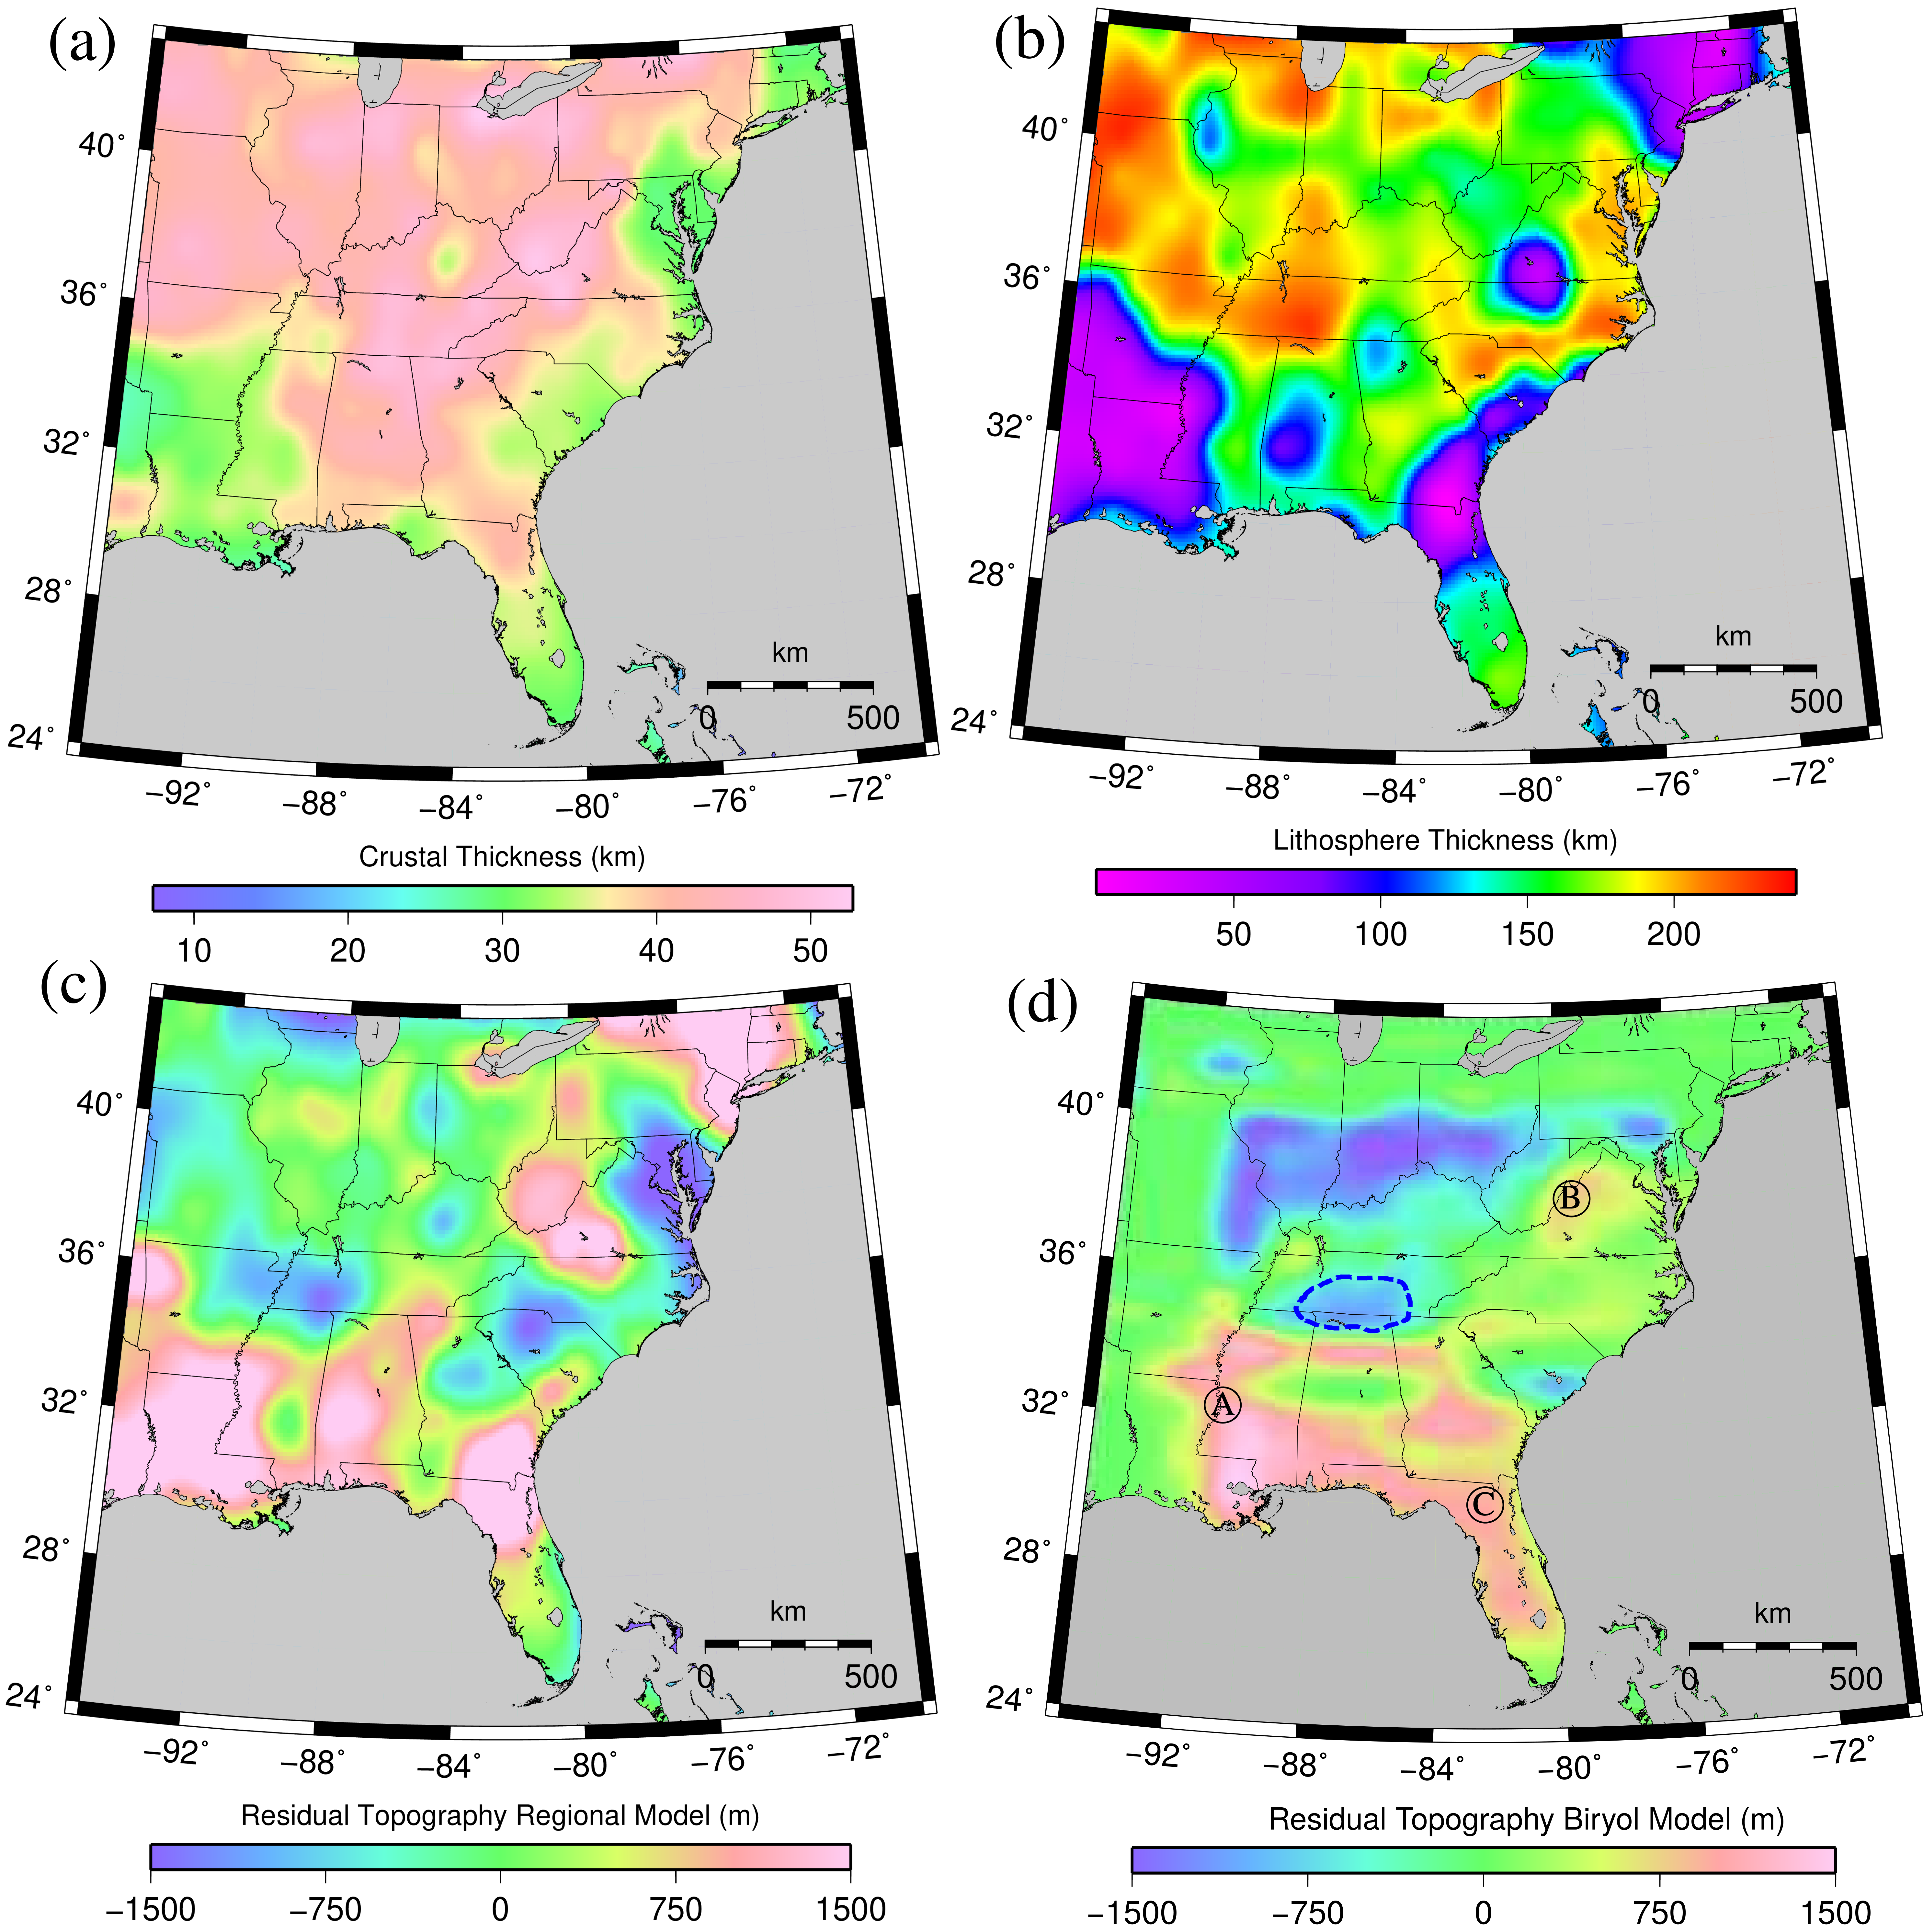
\includegraphics[width=\linewidth]{figures/topography.png}
    \caption{Residual topography calculated from densities based on the regional tomography by~\citet{Biryol_2016} used in this study and from global models. (a) Crustal thickness from CRUST1.0 \citep{laske2013update}. (b) Lithospheric thickness from LITHO1.0~\citep{pasyanos2014litho1} (c) Residual topography calculated using (a) and (b). (d) Residual topography based on the densities calculated using the regional tomography. Encircled letters, A, B, and C, mark the regions where residual topography are strongly positive in both models. The dashed blue line delineates the topographic low due to the lithospheric drip.}%~\citet{Biryol_2016}.}
    \label{topo_res}
\end{figure}

Some similarities are found between the residual topography based on the globally compiled data set (Fig. \ref{topo_res}c) and the one based on the densities calculated from~\citet{Biryol_2016}'s tomography (Fig. \ref{topo_res}d) but these two topography models exhibit inconsistencies as well. The high-density lithospheric drip clearly generates a topographic low (outlined by dashed line in Fig. \ref{topo_res}d). 
%The topographic low is the effect of the density and thickness along depth at each lateral point in the model and, therefore differs from the boundary marked in the Fig.~\ref{fig_temp}. 
Regions marked by encircled letters, A, B, and C on Fig. \ref{topo_res}d show positive dynamic topography coinciding spatially with the positive residual topography in Fig. \ref{topo_res}c although less in extent and magnitudes. The mismatch between the residual and the dynamic topography can be attributed to several factors. Firstly, the seismic tomography puts no constraints on the crustal structure, and the crust is assumed to have a uniform thickness of 40 km to calculate the isostatic response, contrary to the crustal thickness and density variations obtained from the CRUST1.0 model. Secondly, the LITHO1.0 model is about eight times coarser in resolution than the tomography study, and we assumed a constant density of 3300 kg/m$^3$ in the lithosphere instead of the density based on the heterogeneous temperature. We suggest that continued investigation into accurate crustal and lithospheric thickness, and density variations is required to observe any dynamic topography response from the upper mantle flow beneath this region.


The upper mantle heterogeneity results in increased differential stresses at crustal depths and at the CEUS seismic zones. $\Delta \sigma_{\text{diff}}^{\text{HT}-\text{HM}}$ is plotted in Fig.~\ref{df_model}a for the depth of 15 km, at which seismicity in the study area is most frequent~\citep[e.g.,][]{mazzotti2010state}. The seismic zones, ETSZ, SCSZ, GCSZ, CVSZ, and NMSZ are correlated with positive $\Delta \sigma_{\text{diff}}^{\text{HT}-\text{HM}}$ in the range of 30 to 40 MPa (Fig.\ref{df_model}b). The areas F$_{1}$ and F$_{2}$ marked on Fig.\ref{df_model}a do not show active seismicity but $\Delta \sigma_{\text{diff}}^{\text{HT}-\text{HM}}$ is greater than 70 MPa. In contrast, $\Delta\sigma_{\text{diff}}^{\text{HT}-\text{HR}}$ shows only small positive values, 2 to 4 MPa in the horseshoe-shaped region surrounding the drip, which partially overlaps with the ETSZ and NMSZ (Fig.\ref{df_model}b).
%
\begin{figure}[h!]
    \centering
    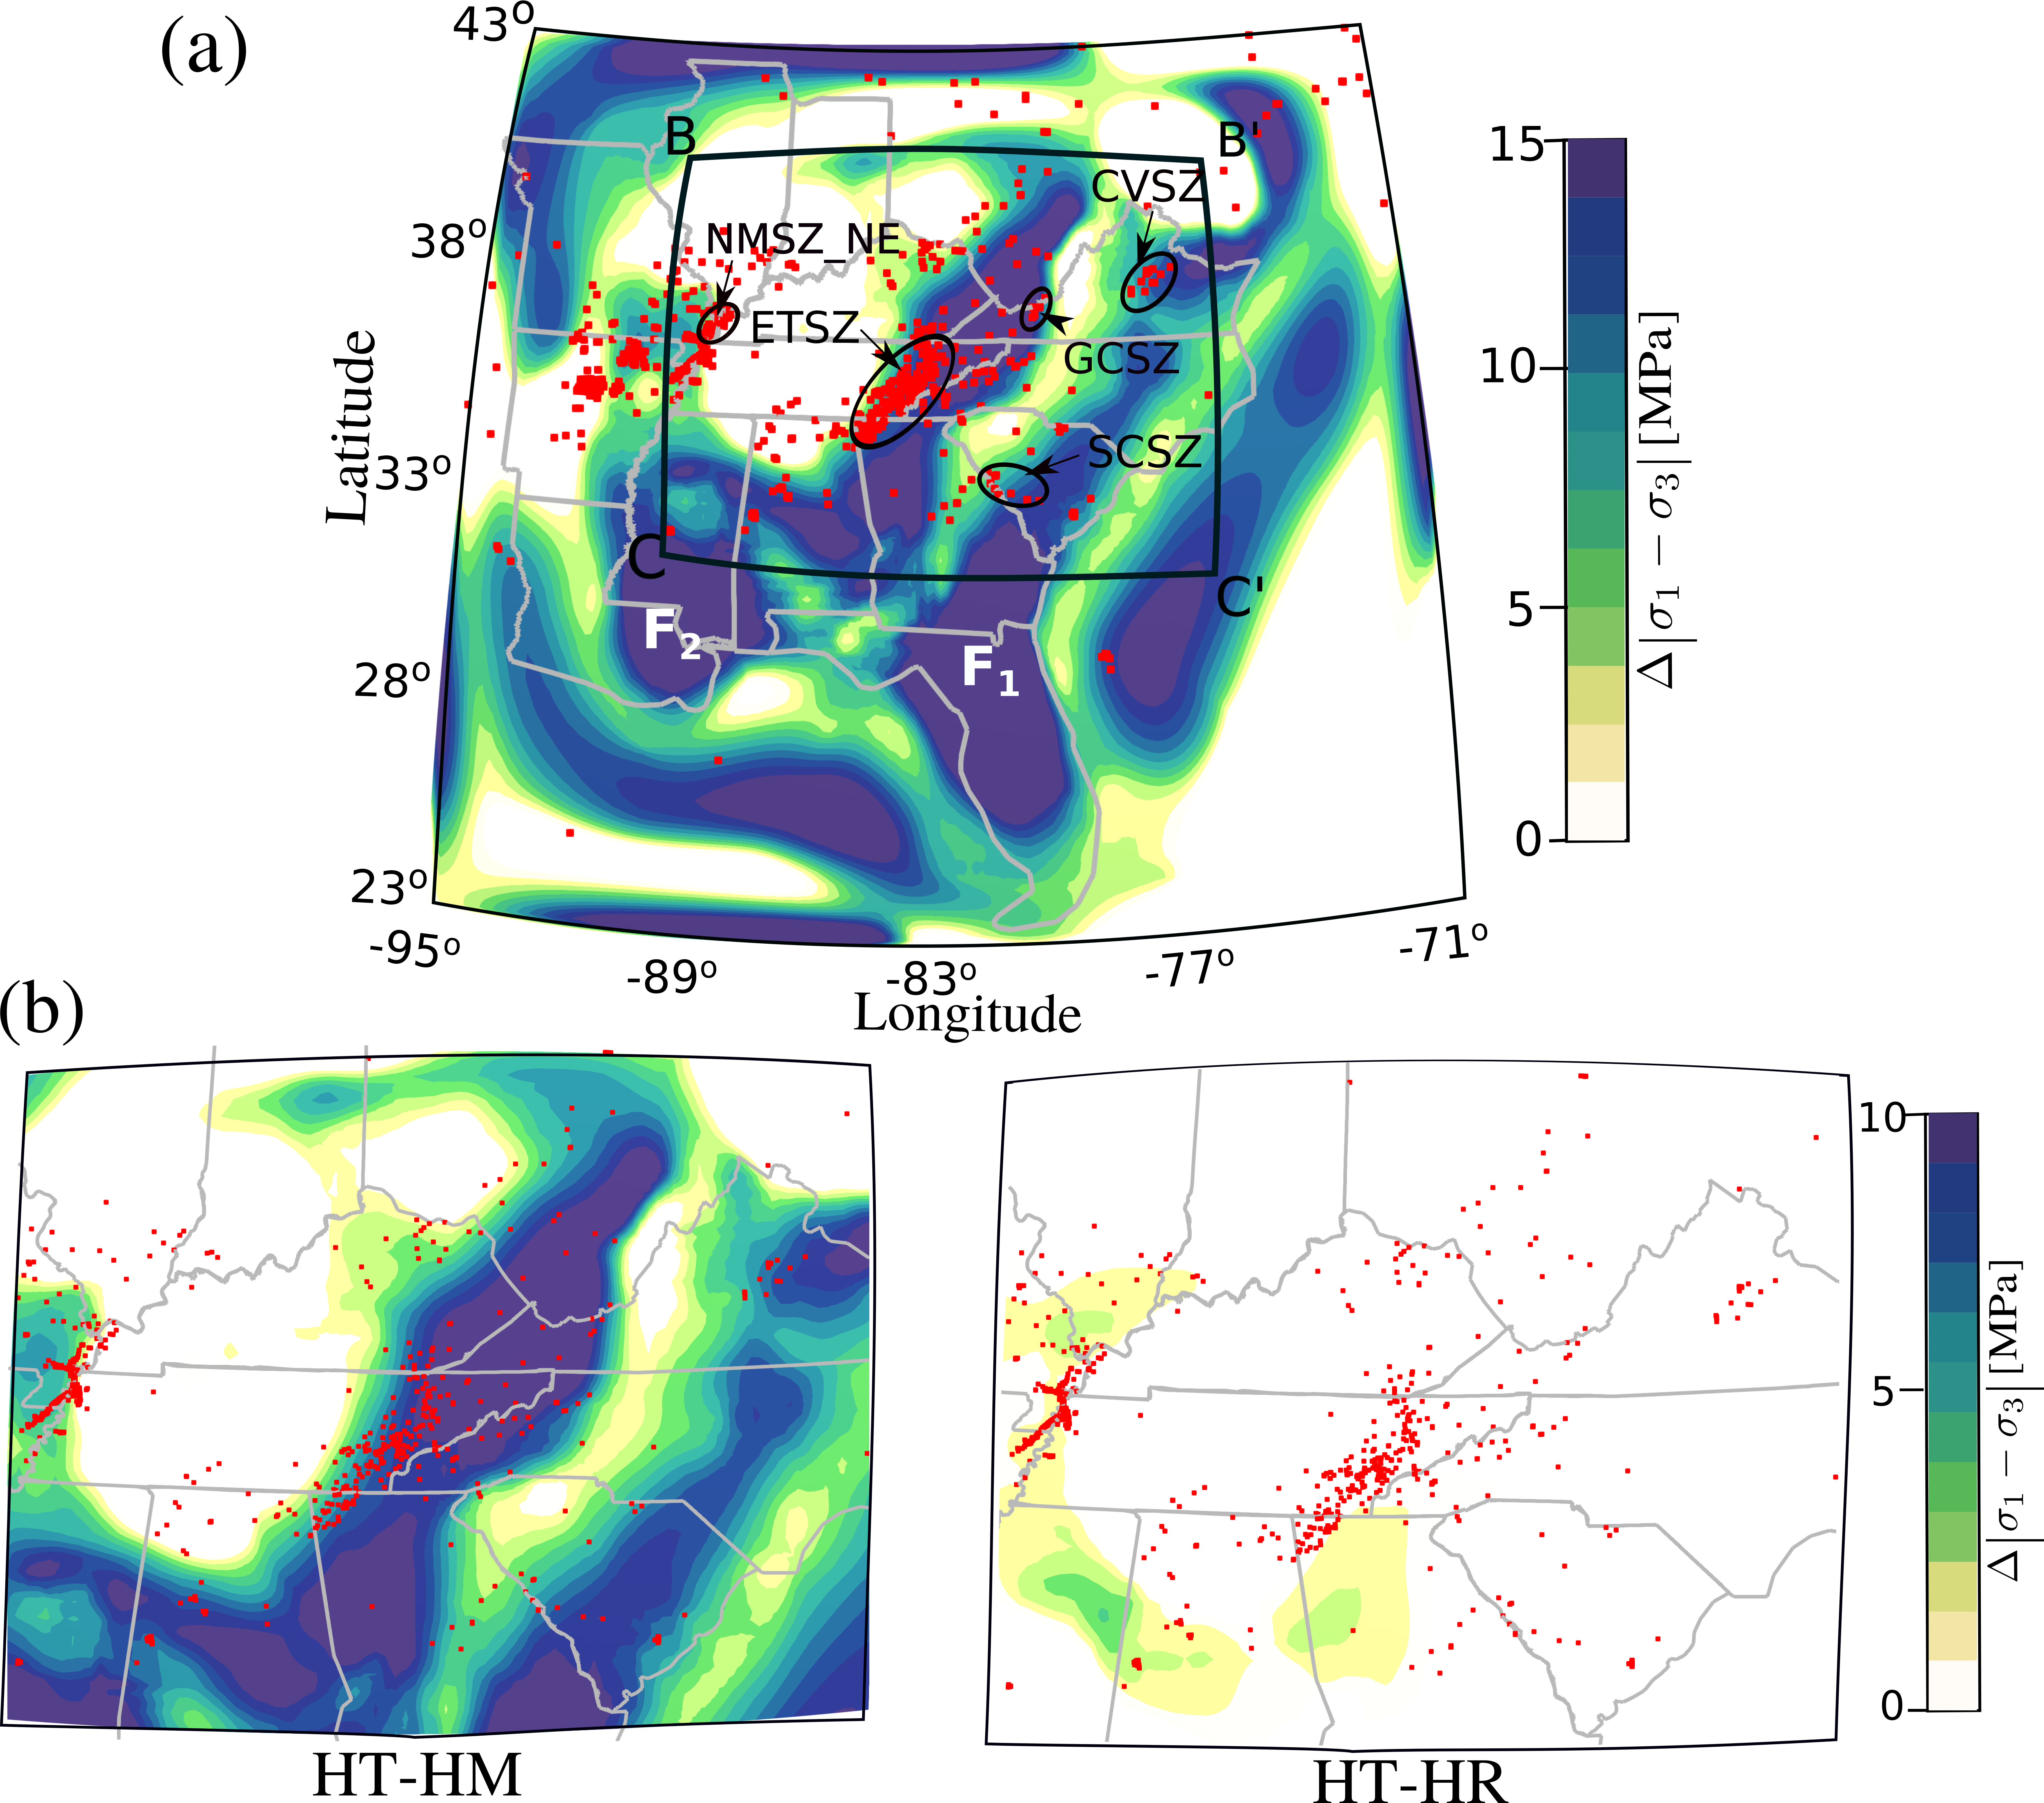
\includegraphics[width=\linewidth]{figures/diff_stress_model.png}
    \caption{(a) Differential stress changes in the HT$-$HM case ($\Delta \sigma_{\text{diff}}^{\text{HT}-\text{HM}}$) at a depth of 15 km. Black dots are earthquake epicenters from USGS data between 2011-2018. Gray lines denote the US state boundaries. Seismic zones investigated in this study are the New Madrid Seismic Zone (NMSZ), Eastern Tennessee Seismic Zone (ETSZ), South Carolina Seismic Zone (SCSZ), Giles County Seismic Zone (GCSZ) and Central Virginia Seismic Zone (CVSZ). F$_1$ and F$_2$ indicates the areas of anomalously high values of $\Delta \sigma_{\text{diff}}^{\text{HT}-\text{HM}}$. Dashed magenta line marks the boundary of the foundering at 605 km depth. The box BB'CC' indicates the region enlarged in subsequent figures. (b) Differential stress change for HT$-$HR ($\Delta \sigma_{\text{diff}}^{\text{HT}-\text{HR}}$) in a region centered on the ETSZ. }
    \label{df_model}
\end{figure}
%
The presence of upper mantle heterogeneity increases the Coulomb stress in  all of the seismic zones for their respective optimal fault orientations listed in Table~\ref{table_fault}. $\Delta \sigma_{\text{diff}}^{\text{HT}-\text{HM}}$, Coulomb stress changes for HT$-$HM are about 5 MPa in the GCSZ and in the  ETSZ for their optimal fault orientations (Fig.~\ref{ht_hm_cs}a). On the other hand, $\Delta$C$_{\text{HT}-\text{HM}}$  for a vertical right-lateral fault striking N10$^{\circ}$E 
indicates that the mantle heterogeneities reduce the slip tendency in the ETSZ but slightly increase it in the NMSZ\_NE (Fig.~\ref{ht_hm_cs}b). 
$\Delta \sigma_{\text{diff}}^{\text{HT}-\text{HM}}$ is about 20 MPa for the thrust motion on the dominant fault orientations in the CVSZ and the SCSZ (Fig.~\ref{ht_hm_cs}c,d). 

\begin{figure}[h!]
    \centering
    \includegraphics[width=0.75\linewidth]{figures/cs_ht_hm.png}
    \caption{Coulomb stress change ($\Delta$C) for HT$-$HM calculated for different fault orientations in Table~\ref{table1}) at 15 km depth. Seismic zone(s) and their corresponding optimal fault geometries are mentioned for each subplot: (a) Eastern Tennessee Seismic Zone (ETSZ) and Giles County Seismic Zone (GCSZ), left lateral vertical fault striking EW, (b) ETSZ and North-eastern arm of the New Madrid Seismic Zone (NMSZ\_NE) and right lateral vertical fault strikingt N10$^\circ$E, (c) Central Virginia Seismic Zone (CVSZ) and thrust fault dipping 50$^\circ$ SE striking N30$^\circ$E, (d) South Carolina Seismic Zone (SCSZ) and thrust fault dipping 40$^\circ$ W striking N-S.}	
    \label{ht_hm_cs}
\end{figure}

Coulomb stress changes due to the lithospheric drip ($\Delta$C$_{\text{HT}-\text{HR}}$) are mostly negative or weakly positive at all the seismic zones for their respective dominant fault orientations (Fig.~\ref{ht_hr_cs}). $\Delta$C$_{\text{HT}-\text{HR}}$ tends to be confined to an area surrounding the drip making relatively greater impact on the ETSZ and NMSZ than on the other seismic zones further east. $\Delta$C$_{\text{HT}-\text{HR}}$ is about 1-2 MPa in the NMSZ\_NE for its dominant fault orientations (Fig. \ref{ht_hr_cs}b) but decreases at the ETSZ for both of the dominant orientations (Fig.~\ref{ht_hr_cs}a, b). The GCSZ, CVSZ and SCSZ are located too far from the drip to have significant $\Delta$C$_{\text{HT}-\text{HR}}$ (Fig.~\ref{ht_hr_cs}a, c and d).

\begin{figure}[ht]
    \centering
    \includegraphics[width=0.75\linewidth]{figures/cs_ht_hr.png}
    \caption{Same as Fig.~\ref{ht_hm_cs} but for HT$-$HR.}
    \label{ht_hr_cs}
\end{figure}
